\documentclass[11pt, a4paper]{book}

\usepackage{mathpazo}
\usepackage[utf8]{inputenc}
\usepackage[T1]{fontenc}
\usepackage{amsmath}
\usepackage{amsfonts}
\usepackage{amssymb}
\usepackage{amsthm}
\usepackage[colorlinks=true, pagebackref=true]{hyperref}
\usepackage[alphabetic]{amsrefs}
\usepackage{mathtools}
\usepackage{xcolor}
\usepackage{titlesec} %reasonable chapter headings
\usepackage{stmaryrd} %double brackets
\usepackage{tikz}
\usepackage[toc,page]{appendix}
\usepackage{listings}
%\usepackage{showlabels}
\usepackage{geometry}

\lstset{language=Python,
backgroundcolor=\color{gray!20},
numberstyle=\footnotesize,
breaklines=true,
basicstyle=\footnotesize,
keywordstyle=\bfseries\color{blue},
commentstyle=\itshape\color{purple},
%identifierstyle=\color{blue},
stringstyle=\color{orange}}
\usetikzlibrary{arrows,positioning,through,decorations.pathmorphing, decorations.markings}

\usepackage{chngcntr}
\counterwithout{equation}{section} %this fixes equation numbering

\titleformat{\chapter}[display]
  {\normalfont\bfseries}{}{0pt}{\Huge} %this eliminates the 'Chapter n' heading

\hypersetup{linkcolor=teal, citecolor=teal}

\def\noteson{%
\gdef\note##1{\marginpar[##1]{##1}}}
\gdef\notesoff{\gdef\note##1{}}
\noteson

\renewcommand\bibname{References}

\newcommand{\NN}{\mathbb{N}}
\newcommand{\ZZ}{\mathbb{Z}}
\newcommand{\QQ}{\mathbb{Q}}
\newcommand{\RR}{\mathbb{R}}
\newcommand{\CC}{\mathbb{C}}

\newcommand{\kQ}{k\langle Q\rangle}
\newcommand{\KQ}{k\langle\!\langle Q\rangle\!\rangle}
\newcommand{\cyc}{\mathrm{cyc}}
\newcommand{\cf}{\mathrm{cf}}
\newcommand{\FA}{k\langle x_1,\dots,x_n\rangle}
\newcommand{\mon}{\langle X\rangle}
\newcommand{\irr}{k\langle X\rangle_{\mathrm{irr}}}
\newcommand{\llangle}{\langle\!\langle}
\newcommand{\rrangle}{\rangle\!\rangle}

\DeclareMathOperator{\End}{End}
\DeclareMathOperator{\Ext}{Ext}
\DeclareMathOperator{\gr}{gr}
\DeclareMathOperator{\Inn}{Inn}

\tikzset{->-/.style={decoration={
  markings,
  mark=at position #1 with {\arrow{>}}},postaction={decorate}}}

\newcommand{\Square}[2]{
\draw (-1+#1, -1+#2) to (-1+#1, 1+#2); %left vertical line
\draw (1+#1, -1+#2) to (1+#1, 1+#2); %right vertical line
\draw (-1+#1, 1+#2) to (1+#1, 1+#2); %top horizontal line
\draw (-1+#1, -1+#2) to (1+#1, -1+#2); %bottom horizontal line
}

\newcommand{\DSquare}[2]{
\draw (-1+#1, -1+#2) to (-1+#1, 1+#2); %left vertical line
\draw (1+#1, -1+#2) to (1+#1, 1+#2); %right vertical line
\draw (-1+#1, 1+#2) to (1+#1, 1+#2); %top horizontal line
\draw (-1+#1, -1+#2) to (1+#1, -1+#2); %bottom horizontal line
\draw (-1+#1, -1+#2) to (1+#1, 1+#2); %diagonal
}

\newcommand{\ArrowedSquare}[2]{
\draw (-1+#1, -1+#2) to (-1+#1, 1+#2); %left vertical line
\draw (1+#1, -1+#2) to (1+#1, 1+#2); %right vertical line
\draw (-1+#1, 1+#2) to (1+#1, 1+#2); %top horizontal line
\draw (-1+#1, -1+#2) to (1+#1, -1+#2); %bottom horizontal line
\draw (-1+#1, -1+#2) to (1+#1, 1+#2); %diagonal
\draw[->, red, very thick] (0.1+#1, -0.9+#2) to (0.9+#1, -0.1+#2); %a
\draw[->, red, very thick] (0.9+#1, #2) to (0.1+#1, #2); %b
\draw[->, red, very thick] (#1, 0.1+#2) to (#1, 0.9+#2); %c
\draw[->, red, very thick] (-0.1+#1, 0.9+#2) to (-0.9+#1, 0.1+#2); %d
\draw[->, red, very thick] (-0.9+#1, #2) to (-0.1+#1, #2); %e
\draw[->, red, very thick] (#1, -0.1+#2) to (#1, -0.9+#2); %f
}

\newcommand\claim[2][.8]{%
  \begin{minipage}{#1\displaywidth}%
  \itshape
  #2
  \end{minipage}%
}

\theoremstyle{plain}
\newtheorem{prop}{Proposition}[chapter]
\newtheorem{lemma}[prop]{Lemma}
\newtheorem{thm}[prop]{Theorem}
\newtheorem{obs}[prop]{Observation}
\theoremstyle{definition}
\newtheorem{exmp}[prop]{Example}
\newtheorem{heur}[prop]{Heuristic}

\begin{document}

\thispagestyle{empty}

\begin {center}


\includegraphics[scale=.3]{uba2.jpg}

\medskip
\textbf{UNIVERSIDAD DE BUENOS AIRES}

\smallskip

\textbf{Facultad de Ciencias Exactas y Naturales}

\smallskip

\textbf{Departamento de Matem\'atica}

\vspace{3.5cm}

\textbf{\large Tesis de Licenciatura}


\vspace{1.5cm}

\textbf{\LARGE Álgebras Jacobianas a través del Lema del Diamante}

\vspace{1.5cm}


\textbf{\large Fernando Daniel Martin}

\end {center}


\vspace{1.5cm}

\noindent \textbf{Director:} Mariano Su\'arez-\'Alvarez


\vspace{3cm}

\rightline{ Fecha de Presentaci\'on}



\tableofcontents
\begin{chapter}*{Introducción}
Un problema recurrente en diversas áreas del álgebra consiste en, dados un objeto algebraico $A$ y un subobjeto $B$, poder entender la estructura del cociente $A/B$. En su trabajo seminal \cite{Ber78}, Bergman introduce el \emph{lema del diamante}, una técnica para poder atacar este problema en el contexto de la teoría de $k$-álgebras. Esencialmente, uno puede entender a las relaciones dadas por los elementos del ideal $B$ como reglas de reescritura para elementos del cociente $A/B$. Si el sistema de reglas de reescritura verifica una cierta condición de confluencia, entonces somos capaces de realizar cómputo explícito en el cociente de una manera sumamente sencilla.

El lema del diamante de Bergman es un resultado muy versátil; en la misma publicación donde fue enunciado aparecen diversas versiones del mismo para múltiples estructuras algebraicas. Más recientemente, en \cite{SAV15} se describe un resultado análogo para completaciones de $k$-álgebras. En este trabajo empleamos esta variación para estudiar una familia particular de cocientes de este tipo de objetos.

En \cite{DWZ08} se describe un procedimiento que permite asignarle un \emph{quiver con potencial}, o \emph{QP}, a una triangulación de una superficie. Un quiver es un multigrafo dirigido, y un potencial es una combinación lineal de ciclos en la completación del álgebra de caminos asociada al quiver. El \emph{álgebra Jacobiana} asociada al QP es un cociente particular de dicha completación; explícitamente, es aquel que se obtiene al cocientar el ideal cerrado generado por las derivadas cíclicas del potencial. En trabajos como \cite{Lad12} y \cite{TVD12} se estudia el problema de determinar si las álgebras Jacobianas procedentes de triangulaciones de superficies cerradas son de dimensión finita. En dichas publicaciones se establece que esto es válido, con la única posible excepción de la esfera con cuatro punciones. En esta tesis estudiamos este tipo de problemas, pero empleando como herramienta principal el lema del diamante. Además, introducimos un procedimiento análogo para generar un QP a partir de una subdivisión poligonal arbitraria de una superficie y abordamos este mismo tipo de problemas en esta nueva situación.

Nuestro trabajo se organiza de la siguiente manera. En el primer capítulo introducimos los preliminares necesarios para definir con precisión los QPs asociados a una triangulación de una superficie, y sus correspondientes álgebras Jacobianas. En el segundo capítulo introducimos el lema del diamante de Bergman en su versión para $k$-álgebras y luego en una variante para completaciones de álgebras de caminos, que será la que usaremos principalmente. Incluimos además varios ejemplos para ilustrar cómo se utiliza el lema del diamante en situaciones concretas.

El tercer capítulo contiene los resultados principales de la tesis. Comenzamos estudiando el caso de la esfera con cuatro punciones, que era el único caso sin cubrir en \cite{Lad12}, y determinamos que el álgebra Jacobiana asociada es de dimensión infinita (más aún, calculamos su serie de Hilbert). Luego, estudiamos el problema de la finito-dimensionalidad en el caso de álgebras Jacobianas procedentes de subdivisiones arbitrarias. Construimos familias infinitas de dichas álgebras tanto de dimensión finita como infinita, mostrando que la situación en el caso poligonal es remarcablemente diferente al caso triangular. Finalmente, producimos sistemas de reescritura confluentes para tres familias de subdivisiones poligonales de la esfera: las pirámides, los prismas y los antiprismas. Las pirámides proveen además de una familia de contraejemplos a la generalización de un teorema de Ladkani (concerniente a la relación entre la dimensión del álgebra y la elección de escalares en el potencial) al caso poligonal.

En el último capítulo, utilizamos estos sistemas de reescritura para calcular invariantes de tipo cohomológico para sus álgebras Jacobianas asociadas. En particular, computamos el centro de dichas álgebras y probamos que admiten derivaciones no triviales.

Finalmente, incluimos un apéndice en el que anexamos y explicamos el funcionamiento de un programa escrito en \texttt{SageMath}, el cual desarrollamos para facilitar el cálculo de sistemas de reescritura.
\end{chapter}
\begin{chapter}*{Introduction}
A recurring problem in various branches of algebra consists in, given an algebraic object $A$ and a subobject $B$, understanding the structure of the quotient $A/B$. In his influential work \cite{Ber78}, Bergman introduces the \emph{diamond lemma}, a tool used to tackle this problem in the context of $k$-algebras. Essentially, one may think of the relations given by elements in the ideal $B$ as rewriting rules for the elements in the quotient $A/B$. If the set of rewriting rules verifies a certain confluence condition, then we are able to carry out explicit computations in the quotient in a simple fashion.

Bergman's diamond lemma is a very versatile result; there are several versions of it for various algebraic structures on the same paper where it was first stated. More recently, in \cite{SAV15}, an analogous result for completions of $k$-algebras is described. In this work, we make use of this variation to study a particular family of quotients of this kind of objects.

In \cite{DWZ08}, the authors describe a procedure that assigns a \emph{quiver with potential}, or \emph{QP} for short, to a triangulation of a surface. A quiver is a directed multigraph, and a potential is a linear combination of cycles in the completion of the path algebra associated to said quiver. The \emph{Jacobian algebra} associated to the QP is a particular quotient of said completion; explicitly, it is the one obtained after modding out the closed ideal spanned by the set of cyclic derivatives of the potential.

In works such as \cite{Lad12} and \cite{TVD12}, the authors determine a key property of these objects: the Jacobian algebra induced by a QP associated to a triangulation of a surface $\Sigma$ is finite-dimensional if $\Sigma$ is not a sphere with four punctures. In particular, the finite-dimensionality of the algebra is independent of the choice of scalars in the potential. 

In this thesis we study this kind of problems, but using the diamond lemma as our main tool. Moreover, we introduce a procedure that assigns a QP to an arbitrary polygonal subdivision of a surface, and we tackle the same kind of problems in this new setting.

Our work is organized as follows. In the first chapter we introduce the necessary preliminaries in order to define the QP associated to a triangulation of a surface, and its corresponding Jacobian algebra. In the second chapter we introduce Bergman's diamond lemma, first in the classical $k$-algebra setting and then we present a variation of it that applies over completions of path algebras, which we will use the most. We also include several examples, with the purpose of showing how the diamond lemma is used in concrete situations.

The third chapter contains our main results. We start off by studying the case of the sphere with four punctures, which is the only case not discussed in \cite{Lad12}, and we prove that the associated Jacobian algebra is infinite-dimensional (moreover, we compute its Hilbert series). We then study the finite-dimensionality problem in the case of Jacobian algebras arising from arbitrary polygonal subdvisions. We construct infinite families of said algebras, of both finite and infinite dimension, showing that the situation in the polygonal case is remarkably different to the triangular case. Finally, we produce confluent rewriting systems for three families of polygonal subdivisions of the sphere: pyramids, prisms and antiprisms. Pyramids also provide a family of counterexamples to the generalization of a theorem of Ladkani (concerning the relation between the dimension of the Jacobian algebra and the choice of scalars appearing in the potential) to the polygonal case.

In the last chapter, we use these rewriting systems to compute cohomological invariants of the associated Jacobian algebras. In particular, we compute the center of said algebras and we prove that they admit non-trivial derivations.

Finally, we include an appendix on which we present a program written in \texttt{SageMath}, which we developed to ease computations related to rewriting systems.
\end{chapter}
\begin{chapter}{Preliminaries}
Throughout the text, $k$ will denote a field of characteristic zero.
\begin{section}{The path algebra of a quiver}
A \emph{quiver} is a quadruple $Q=(Q_0, Q_1, s,t)$, where $Q_0$ and $Q_1$ are finite sets whose elements are called \emph{vertices} and \emph{arrows} respectively, and $s,t:Q_1\to Q_0$ are functions that associate to each arrow $\alpha\in Q_1$ its \emph{source} $s(\alpha)\in Q_0$ and its \emph{target} 
$t(\alpha)\in Q_0$. We will usually abbreviate the fact that an arrow $\alpha\in Q_1$ has source $a$ and target $b$ using the notation $\alpha:a\to b$. We will also omit mentioning $s$ and $t$ explicitly when they are clear from context.

One can represent a quiver graphically as an oriented graph allowing loops and multiple arrows between the same pair of vertices. The following are some examples of quivers:
\[
\begin{tikzpicture}[->, node distance=1cm, thick, auto]
\tikzstyle{every node} = [circle, fill=gray!30, minimum size=.5cm]
\tikzset{every loop/.style={looseness=15}}
\node (a) at (0:1) {};
\node (b) at (120:1) {};
\node (c) at (240:1) {};
\path (a) edge [bend right] (b)
(b) edge [bend right] (c)
(c) edge [bend right] (a)
(a) edge [in=15, out=-15, loop] (a)
(b) edge [in=135, out=105, loop] (b)
(c) edge [in=255, out=225, loop] (c);
\node (d) [right=of a,xshift=2cm] {};
\node (e) [right=of d] {};
\foreach \from/\to in {d/e, e/d}
\draw (d.40) -- (e.140);
\draw (e) -- (d);
\draw (d.320) -- (e.220);
\end{tikzpicture}
\]
\[
\begin{tikzpicture}[->,node distance=1cm, thick]
\tikzstyle{every node} = [circle, fill=gray!30, minimum size=.5cm]
\node (1) {};
\node (2) [right=of 1] {};
\node (3) [right=of 2] {};
\node (4) [right=of 3] {};
\node (5) [right=of 4] {};
\node (6) [right=of 5] {};
\node (7) [right=of 6] {};
\node (8) [below=of 3] {};
\foreach \from/\to in {2/1, 3/2, 3/4, 3/8, 4/5, 5/6, 6/7}
\draw [->] (\from) -- (\to);
\end{tikzpicture}
\]
Let $Q=(Q_0, Q_1, s, t)$ be a quiver and consider the $k$-vector spaces $R=k^{Q_0}$ and $A=k^{Q_1}$, which we will call the \emph{vertex span} and \emph{arrow span} of $Q$, respectively. The space $R$ is a commutative $k$-algebra with the product given by pointwise multiplication. Thus, we can consider an $R$-bimodule structure on $A$ given as follows: if $r\in Q_0$, $\alpha\in Q_1$ then we define $r\alpha = \delta_{r,t(\alpha)} \alpha$ and analogously $\alpha r = \delta_{r, s(\alpha)}\alpha$, and extend the action linearly. Therefore, a vertex $r$ acts as the identity on the left (right) of an arrow $\alpha$ if the target (source) of $\alpha$ is $r$, and otherwise acts as zero. The \emph{path algebra} $\kQ$ associated to the quiver $Q$ is the graded tensor algebra
\[
\kQ = \bigoplus_{n=0}^\infty A^{\otimes_R n},
\]
where we set $A^{\otimes_R 0}=R$. For the sake of simplicity we will usually notate $A^{\otimes_R n}$ as $A^n$ and an elementary tensor $\alpha_n\otimes\dots\otimes \alpha_1$ as $\alpha_n\dots\alpha_1$. Notice that a non-zero element of the form $\alpha_n\dots\alpha_1$ consists of a sequence of \emph{concatenable} arrows $\alpha_i$, that is, arrows such that $s(\alpha_{i+1})=t(\alpha_i)$. We will call such an element a \emph{path of length n}. It is worth observing that the collection of all paths of length $n$ form a basis of $A^n$ as a $k$-vector space. Since $Q_0$ is a basis of $A^0=R$, we will refer to elements of $Q_0$ as \emph{paths of length 0}, which we will usually call \emph{trivial} or \emph{stationary} paths. Considering $Q_0$ and $Q_1$ are in bijection with paths of length 0 and 1 respectively, we will denote the set of paths of length $n$ as $Q_n$ and the set of all paths as $Q_*$. We can now define source and target functions $s,t:Q_*\to Q_0$ as follows: if $u=\alpha_n\dots\alpha_0\in Q_n$ with $n>0$, then $s(u)=s(\alpha_0)$ and $t(u)=t(\alpha_n)$. Otherwise, if $u=r\in Q_0$ then $s(u)=t(u)=r$. Thus, one easily checks that if $a,b\in Q_0$, the space spanned by paths with source $a$ and target $b$ is exactly $b\kQ a$.

The path algebra satisfies the following useful universal property:

\begin{prop} Let $Q$ be a quiver and $\Lambda$ be an associative $k$-algebra with unit. Suppose $f_0:Q_0\to \Lambda$, $f_1:Q_1\to\Lambda$ are maps satisfying:
\begin{enumerate}
\item $\sum_{r\in Q_0} f_0(r)=1$.
\item If $a\in Q_0$, then $f_0^2(a)=f_0(a)$.
\item If $a\neq b\in Q_0$, then $f_0(a)f_0(b)=0$.
\item If $\alpha:a\to b$ is an arrow in $Q_1$, then $f_1(\alpha) = f_0(b) f_1(\alpha) f_0(a)$.
\end{enumerate}
Then, there exists a unique $k$-algebra morphism $f:\kQ\to \Lambda$ extending $f_0$ and $f_1$.
\end{prop}
\begin{proof} If $n\geq 1$, define $f(\alpha_n\dots\alpha_1)=f_1(\alpha_n)\dots f_1(\alpha_0)$ and let $f(r)=f_0(r)$ for $r\in Q_0$. As the set of all paths forms a basis of $\kQ$ as a vector space, this defines a $k$-linear map $f:\kQ\to \Lambda$. Condition 1 guarantees that such a map preserves the unit and conditions 2, 3 and 4 guarantee that it preserves products involving stationary paths. Since by definition $f$ preserves products of non-trivial paths, we conclude that $f$ is a $k$-algebra morphism extending $f_0$ and $f_1$. As for uniqueness, consider another extension $g:\kQ\to\Lambda$. Since $g$ is a $k$-algebra morphism, we have that $g(\alpha_n\dots\alpha_1)= g(\alpha_n)\dots g(\alpha_1)= f_1(\alpha_n)\dots f_1(\alpha_1)=f(\alpha_n\dots\alpha_1)$ for $n\geq 1$ and $g(r)=f_0(r)=f(r)$ for all $r\in Q_0$. Thus $g$ agrees with $f$ in a basis, and so $g=f$ as wanted.
\end{proof}
Let us now consider some examples:
\begin{exmp} Let $Q$ be the quiver with vertices $\{1,\dots,n\}$ and no arrows:
\[
\begin{tikzpicture}[node distance=1cm, auto, thick]
\tikzstyle{every node} = [circle, fill=gray!30, minimum size=.5cm, inner sep=.07cm]
\node (1) {1};
\node (2) [right=of 1] {2};
\node (3) [right=of 2] {3};
\node (4) [right=of 3, fill=white] {...};
\node (5) [right=of 4] {n};
\end{tikzpicture}
\]
The path algebra $\kQ$ is then isomorphic to $k^n = ke_1\oplus\dots\oplus ke_n$, where multiplication is given by $e_i e_j = \delta_{i,j} e_i$ and extended linearly.
\end{exmp}

\begin{exmp}\label{one-loop} Let $Q$ be the quiver with a single vertex $1$ and a single arrow $\alpha:1\to 1$:
\[
\begin{tikzpicture}[->, thick]
\tikzset{every loop/.style={looseness=15}}
\node[circle, fill=gray!30, minimum size=.5cm, inner sep=.07cm]  (1) {1};
\path (1) edge [loop above] node {$\alpha$} (1);
\end{tikzpicture}
\]
The path algebra $\kQ$ has a basis given by $\{e_a, \alpha, \alpha^2, \dots\}$. It is easily seen that $\kQ$ is isomorphic to the polynomial algebra $k[x]$, via the map sending $\alpha \mapsto x$ and $1\mapsto 1$.
\end{exmp}
\begin{exmp}\label{several-loops} More generally, let $Q$ be the quiver with a single vertex $1$ and $n$ arrows $\alpha_n:1\to 1$:
\[
\begin{tikzpicture}[->, auto, thick]
\tikzset{every loop/.style={looseness=15}}
\node[circle, fill=gray!30, minimum size=.5cm, inner sep=.07cm]  (1) {1};
\node[circle, fill=white] (2) at +(270: 1) {...};
\path (1) edge [loop left] node {$\alpha_5$} (1);
\path (1) edge [loop above] node {$\alpha_3$} (1);
\path (1) edge [loop right] node {$\alpha_1$} (1);
\path (1) edge [in=30, out=60, loop] node {$\alpha_2$} (1);
\path (1) edge [in=210, out=240, loop] node {$\alpha_6$} (1);
\path (1) edge [in=120, out=150, loop] node {$\alpha_4$} (1);
\path (1) edge [in=300, out=330, loop] node {$\alpha_n$} (1);
\end{tikzpicture}
\]
Then, the path algebra $\kQ$ is isomorphic to the free algebra on $n$ generators $k\langle x_1,\dots, x_n\rangle$, via the map sending $\alpha_i\mapsto x_i$ and $1\mapsto 1$.
\end{exmp}

A path $u\in Q_n$ with $n>1$ such that $s(u)=t(u)$ is called a \emph{cycle}, and a quiver containing no cycles is said to be \emph{acyclic}. As we can infer from the previous examples, the existence of cycles in the quiver is closely related to the dimension of the path algebra. More precisely, we have:

\begin{prop}\label{acyclic-fin-dim}
Let $Q$ be a quiver and $\kQ$ its associated path algebra. Then $\kQ$ is finite-dimensional iff $Q$ is acyclic.
\end{prop}
\begin{proof} Suppose $\kQ$ is infinite-dimensional. Then the set of all paths $Q_*$, which is a basis for $\kQ$, must be infinite. Since the quiver has only a finite number of arrows, there's only a finite number of paths of less than a fixed length. Therefore, if the set of paths $Q_*$ is infinite, then there exist arbitrarily long paths. Let $n$ be the number of vertices in $Q_0$ and pick a path $\alpha_m\dots\alpha_1$ with $m>n$. Then $s(\alpha_i) = t(\alpha_j)$ for some $1\leq i < j\leq m$ and so $\alpha_j\dots\alpha_i$ is a cycle in $Q$.

Conversely, if $Q$ contains a cycle $u$, then $\{u,u^2,u^3,\dots\}$ is an infinite linearly independent set, and so $\kQ$ is infinite-dimensional.
\end{proof}

\begin{section}{The Jacobian algebra of a quiver with potential}

\marginpar{\textcolor{red}{motivación}}

Maintaining our previous notation, we now define the \emph{complete path algebra} $\KQ$ associated to a quiver $Q$ as
\[
\KQ = \prod_{n=0}^\infty A^n,
\]
that is, elements of $\KQ$ are possibly infinitely supported linear combinations of paths in $Q_*$ and the product on $\KQ$ is just the natural extension of the product on $\kQ$.

\marginpar{\textcolor{red}{todo este párrafo debería explicarse mejor una vez que esté hecha la parte del lema topológico}}

The path algebra $\kQ$ admits a $k$-algebra ultranorm $\vert \cdot \vert: \kQ\to [0, \infty)$ such that for each non-zero $x=\sum_{u\in Q_*} \lambda_u u$ we have $\vert x\vert = e^{-\nu(x)}$, where $\nu(x) = \min\{ i\in \NN_0 : |u| = i \text{ and } \lambda_u \neq 0 \}$. We call this the \emph{$\mathfrak{m}$-adic ultranorm} on $\kQ$. One can check that the complete path algebra $\KQ$ is in fact the completion of the path algebra $\kQ$ with respect to the $\mathfrak{m}$-adic ultranorm.

It is easy to see that the usual path algebra $\kQ$ is a dense $k$-subalgebra and $R$-subbimodule of $\KQ$.

\marginpar{\textcolor{red}{acá o bien en la parte del lema topológico habría que probar algunas propiedades básicas de la topología -- cuál es la noción de convergencia, etc.}}

We now consider the completions of the examples of path algebras mentioned previously:

\begin{exmp}Let $Q$ be an acyclic quiver. As we proved in \ref{acyclic-fin-dim}, the associated path algebra $\kQ$ is finite-dimensional, and so $A^n=0$ for big enough $n$. Therefore, $\bigoplus A^n=\prod A^n$ and thus the path algebra coincides with its completion.
\end{exmp}

\begin{exmp}Let $Q$ be the quiver from \ref{several-loops}. The isomorphism $\kQ\simeq k\langle x_1,\dots,x_n\rangle$ extends to an isomorphism between the respective completions $\KQ\simeq k\langle\langle x_1,\dots,x_n\rangle\rangle$, where the right-hand side term denotes the algebra of non-commutative formal power series in $n$ variables.
\end{exmp}
\end{section}

Let $\KQ=\prod A^n$ be the complete path algebra associated to a quiver $Q$. For $n\geq 1$, we define the \emph{cyclic part} of $A^n$ as
\[
A^n_{\cyc} = \bigoplus_{r\in Q_0} rA^nr,
\]
that is, the $R$-submodule spanned by cycles of length $n$. A \emph{potential} $S$ is an element of the closed \marginpar{\textcolor{red}{por qué $\KQ_{\cyc}$ es cerrado?}} $R$-submodule $\KQ_{\cyc}\subseteq \KQ$, which we define as
\[
\KQ_{\cyc}=\prod_{n=1}^\infty A^n_{\cyc}
\]
In other words, a potential is a possibly infinitely supported linear combination of cycles. We will call a pair $(Q,S)$ a \emph{quiver with potential}, or \emph{QP} for short.

In their work \cite{RSS80}, Rota, Sagan and Stein introduced a notion of derivative for non-commutative algebras, called the \emph{cyclic derivative}. Here we will work with this concept within the context of the complete path algebra of a quiver. Given an arrow $\alpha\in Q_1$, the cyclic derivative with respect to $\alpha$ is the morphism $\partial_\alpha:\KQ_\cyc\to \KQ$ defined for a cycle $u=\alpha_n\dots\alpha_1$ as
\[
\partial_\alpha(u) = \sum_{k=1}^n \delta_{\alpha, \alpha_k}\alpha_{k+1}\dots\alpha_n\alpha_1\dots\alpha_{k-1}
\]
and extended linearly and continuously.

We are now able to introduce the \emph{Jacobian algebra} associated to a QP, which is the main object of study in this thesis. Given a QP $(Q,S)$, the \emph{Jacobian ideal} $J(S)$ is the closed ideal in $\KQ$ generated by the set of all cyclic derivatives of the potential, that is, $\{\delta_\alpha(S) : \alpha\in Q_1\}$. The Jacobian algebra $P(Q,S)$ is then the quotient $\KQ/J(S)$.

\begin{exmp} As in \ref{one-loop}, consider the quiver $Q$ with a single vertex and a unique arrow from that vertex to itself. As we have seen, the complete path algebra $\KQ$ is isomorphic to the algebra of formal power series $k\llbracket x\rrbracket$. Identifying $x$ with the only arrow in the quiver, we see that any potential for Q is of the form $\sum_{n=1}^\infty \lambda_n x^n$ for some choice of scalars $\lambda_n\in k$. For example, let us consider the potential $S=x^n$. Since $x$ is the only arrow in the quiver, we just have to compute $\partial_x(x^n)$, which turns out to be $nx^{n-1}$ (happily coinciding with the usual, commutative notion of derivation). Therefore, the Jacobian algebra is $k\llbracket x\rrbracket/(nx^{n-1})$, which is isomorphic to the truncated polynomial algebra $k[x]/(x^{n-1})$.
\end{exmp}

Two potentials $S$ and $S'$ are said to be \emph{cyclically equivalent} if their difference $S-S'$ lies in the closed $k$-subspace spanned by elements of the form $\alpha_n\dots\alpha_1 - \alpha_1\alpha_n\dots\alpha_2$ where $\alpha_n\dots\alpha_1$ is a cycle, or equivalently, if every term of $S$ is a cyclic permutation of the factors of a term of $S'$. It is easily checked that if $S$ and $S'$ are cyclically equivalent, then $\partial_\alpha(S)$ is just a reordering of the summands of $\partial_\alpha(S')$, and so they coincide. This in turn implies that $S$ and $S'$ induce both the same Jacobian ideal and the same Jacobian algebra.

If $(Q,S)$ and $(Q', S')$ are QPs sharing the same set of vertices, we say that $(Q,S)$ is \emph{right-equivalent} to $(Q',S')$ if there exists a $k$-algebra isomorphism $\varphi:\KQ\to k\langle\langle Q'\rangle\rangle$ fixing the set of vertices and such that $\varphi(S)$ is cyclically equivalent to $S'$. This will be our concept of isomorphism for QPs, since a right-equivalence induces an isomorphism between the respective Jacobian algebras, as seen in Proposition 3.7 from \cite{DWZ08}.

\begin{exmp} Let $Q$ be the quiver with vertices 1 and 2, and arrows $\alpha:1\to 2$, $\beta:2\to1$:
\[
\begin{tikzpicture}[->,node distance=1cm, thick]
\tikzstyle{every node} = [circle, fill=gray!30, minimum size=.5cm, inner sep=.07cm]
\node (1) {1};
\node (2) [right=of 1] {2};
\foreach \from/\to in {2/1, 1/2}
\draw (1.20) -- (2.160) node[midway, above, fill=white] {$\alpha$};
\draw (2.200) -- (1.340) node[midway, below, fill=white] {$\beta$};
\end{tikzpicture}
\]
Any potential for $Q$ is of the form $\sum_{n=1}^\infty \lambda_n (\alpha\beta)^n + \mu_n (\beta\alpha)^n$ for some scalars $\lambda_n, \mu_n\in k$. For instance, the cyclically equivalent potentials $S=(\alpha\beta)^n$ and $S'=(\beta\alpha)^n$ give rise to the same Jacobian ideal, which is $(\partial_\alpha(S), \partial_\beta(S)) = (n(\beta\alpha)^{n-1}\beta, n(\alpha\beta)^{n-1}\alpha)$. As any path of length at least $n$ has either $(\beta\alpha)^{n-1}\beta$ or $(\alpha\beta)^{n-1}\alpha$ as factors, the Jacobian ideal contains $A^d$ for $d\geq n$. Therefore, the Jacobian algebra $P(Q,S)$ turns out to be finite-dimensional.
\end{exmp}

In the context of Jacobian algebras, having finite dimension is a highly desirable attribute. A usual method for proving this, as seen in the works of \cites{LF09, Lad12, TVD12}, consists in showing that enough cycles are contained in the Jacobian ideal, just as we did in the toy example above. We will make use of the diamond lemma in order to produce this kind of arguments in a streamlined fashion.
\end{section}

\begin{section}{Ideal triangulations of surfaces}
In this thesis we will focus primarily on a family of QPs (and their associated Jacobian algebras) arising from a particular procedure carried out on a triangulation of a \textcolor{red}{Riemann?} surface. In order to do this, we start with some basic definitions regarding our geometric objects.

Throughout the text, we will refer to compact, connected, oriented \textcolor{red}{2-manifolds/Riemann surfaces?} with boundary simply as \emph{surfaces}. We now state a classical result in combinatorial topology that completely classifies these objects:\marginpar{la definición de genus debería ir fuera de la prop?}

\begin{prop}\label{surf-classification} Let $\Sigma$ be a surface with a number $b$ of boundary components. Then $\Sigma$ is homeomorphic to either a sphere with $b$ open disks removed or to a $g$-holed torus with $b$ open disks removed. We call the number $g$ the \emph{genus} of the surface and set $g=0$ in the spherical case.
\end{prop}
\begin{proof} See \cite[Section 10]{Mas77}.
\end{proof}

A \emph{surface with marked points} $(\Sigma,M)$ is an ordered pair consisting of a surface $\Sigma$ and a finite, non-empty collection $M$ of points (called \emph{marked points}) of $\Sigma$ containing at least one point from each of its boundary components. Points in $M$ that belong to the interior of $\Sigma$ are called \emph{punctures}.

An \emph{arc} on a surface with marked points $(\Sigma, M)$ is a curve $\gamma:[0,1]\to \Sigma$ such that:
\begin{enumerate}
\item Its endpoints lie in $M$.
\item Its restriction to $(0,1)$ is injective and does not intersect $M$ or the boundary of $\Sigma$.
\item Its image is not contractible into $M$ or onto the boundary of $\Sigma$.
\end{enumerate}
\begin{figure}[h]
\[
\begin{tikzpicture}[thick]
\tikzstyle{every node} = [circle, fill=black, minimum size=.2cm, inner sep=0cm]
\node (se1) at (0,0) {};
\node (sw1) at (2,0) {}
	edge (se1);
\node (n1) at (1,1.73) {}
	edge (se1)
	edge (sw1);
\node (c1) at (1,0.7) {}
	edge (se1);

\node (se2) at (3,0) {};
\node (sw2) at (5,0) {}
	edge (se2);
\node (n2) at (4,1.73) {}
	edge (se2)
	edge (sw2)
	edge [bend left] (se2);
\node (c2) at (4,0.7) {};

\node (se3) at (6,0) {}
	edge [in=25, out=45, distance=1.1cm] (se3);
\node (sw3) at (8,0) {}
	edge (se3);
\node (n3) at (7,1.73) {}
	edge (se3)
	edge (sw3);
\node (c3) at (7,0.7) {};
\end{tikzpicture}
\]
\caption{While the first is an arc of the punctured triangle, the last two are not, since they are contractible to the boundary or to the set of marked points, respectively.}
\end{figure}

We will consider arcs on a surface only up to isotopy relative to $M$. Two arcs will be said to be \emph{compatible} if there exist representatives in their corresponding relative isotopy classes such that they do not intersect in the interior of $\Sigma$. An \emph{ideal triangulation} for $(\Sigma, M)$ is then a maximal family of compatible arcs in $\Sigma$.

\begin{figure}[h]
\[
\begin{tikzpicture}[thick]
\label{square-triangs}
\tikzstyle{every node} = [circle, fill=black, minimum size=.2cm, inner sep=0cm]
\node (sw1) at (0,0) {};
\node (nw1) at (0,2) {}
	edge (sw1);
\node (se1) at (2,0) {}
	edge (sw1);
\node (ne1) at (2,2) {}
	edge (nw1)
	edge (se1);
\node (c1) at (1,1) {}
	edge (sw1)
	edge (nw1)
	edge (se1)
	edge (ne1);

\node (sw2) at (3,0) {};
\node (nw2) at (3,2) {}
	edge (sw2);
\node (se2) at (5,0) {}
	edge (sw2)
	edge [bend left] (nw2);
\node (ne2) at (5,2) {}
	edge (nw2)
	edge (se2);
\node (c2) at (4,1) {}
	edge (nw2)
	edge (se2)
	edge (ne2);

\node (sw3) at (6,0) {};
\node (nw3) at (6,2) {}
	edge (sw3);
\node (se3) at (8,0) {}
	edge (sw3)
	edge [bend left] (nw3)
	edge [bend right] (nw3);
\node (ne3) at (8,2) {}
	edge (nw3)
	edge (se3);
\node (c3) at (7,1) {}
	edge (nw3)
	edge (se3);

\node (sw4) at (9,0) {};
\node (nw4) at (9,2) {}
	edge (sw4);
\node (se4) at (11,0) {}
	edge (sw4)
	edge [bend left] (nw4)
	edge [bend right] (nw4)
	edge [in=150, out=120,distance=2.4cm] (se4);
\node (ne4) at (11,2) {}
	edge (nw4)
	edge (se4);
\node (c4) at (10,1) {}
	edge (se4);
\end{tikzpicture}
\]
\caption{Some ideal triangulations of the square with one puncture.}
\end{figure}
\marginpar{\textcolor{red}{las figuras no quedan bien ubicadas}}

An ideal triangulation divides the surface $\Sigma$ into \emph{ideal triangles}. As we can see in \ref{square-triangs}\marginpar{por algún motivo eqref muestra 1.3 en vez de 1.2...}, such triangulations are more general than the usual ones, since they admit configurations in which two triangles share more than one side. Even more, the three sides of an ideal triangle may not be distinct. In that case we say that the triangle is \emph{self-folded}.
\begin{figure}[h]
\[
\begin{tikzpicture}[thick]
\tikzstyle{every node} = [circle, fill=black, minimum size=.2cm, inner sep=0cm]
\node (se1) at (0,0) {};
\node (sw1) at (2,0) {}
	edge (se1);
\node (n1) at (1,1.73) {}
	edge (se1)
	edge (sw1);
\node (cbase1) at (4,0) {};
\node [draw,circle through=(cbase1), fill=none] at (4,1) {};
\node (cbase2) at (7,0) {};
\node (cmid2) at (7,1) {}
	edge (cbase2);
\node [draw,circle through=(cbase2), fill=none] at (7,1) {};
\end{tikzpicture}
\]
\caption{The three possible kinds of ideal triangles: the usual \emph{triangle} and the self-folded ones, which are the \emph{monogon} and the \emph{digon}.}
\end{figure}

As one may observe, every ideal triangulation of the square pictured in \ref{square-triangs} \marginpar{\textcolor{red}{la numeración de las figuras debería seguir la de las props?}} consists of exactly 4 arcs. Indeed, the number of arcs in a triangulation is an invariant of the marked surface, which we call its \emph{rank}. More precisely, we have:

\begin{prop}[{\cite[Proposition 2.10]{FST08}}] Any ideal triangulation of a surface with marked points $(\Sigma, M)$ consists of exactly
\[
n=6g+3b+3p+c-6
\]
arcs, where $g$ is the genus of the surface $\Sigma$, $b$ is its number of boundary components, $p$ is the number of punctures and $c$ is the number of marked points lying on the boundary.
\end{prop}
\begin{proof} One can show using the classification theorem \ref{surf-classification} that the Euler characteristic of a surface $\Sigma$ of genus $g$ with $b$ boundary components is
\begin{equation}\label{euler-ch1}
\chi(\Sigma)=2-2g-b
\end{equation}
On the other hand, we can compute the Euler characteristic of the surface regarding an ideal triangulation as a cellular decomposition. Since an ideal triangulation is a maximal collection of compatible arcs, any marked point must be a vertex of the decomposition and so we have $v = c + p$ vertices. As for edges, we have $n$ of them in the interior of the surface and $c$ of them in the boundary, which amounts to $e = n + c$. Finally, we know that each face is triangular, that any edge in the interior of the surface belongs to two different faces, and that edges in the boundary belong to only one face. Therefore, by counting faces we arrive at $3f = 2n+c$. Putting it all together, we get that
\begin{equation}\label{euler-ch2}
\chi(\Sigma)=v-e+f=(c+p)-(n+c)+\left(\frac{2}{3}n+\frac{1}{3} c\right)=p+\frac{1}{3}(c-n)
\end{equation}
The result now follows by equating \eqref{euler-ch1} and \eqref{euler-ch2} and solving for $n$.
\end{proof}

From now on, we will assume that our surface $(\Sigma, M)$ is none of the following:
\begin{enumerate}
\item A sphere with one, two or three punctures.
\item An unpunctured or once-punctured monogon.
\item An unpunctured digon.
\item An unpunctured triangle.
\end{enumerate}
The reason for these exclusions is that the listed surfaces either have no non-trivial triangulations or only have pathological ones. In fact, we have the following result:

\begin{prop}[{\cite[Proposition 2.13]{FST08}}] Let $(\Sigma, M)$ be any surface with marked points not on the list above. Then $(\Sigma, M)$ admits an ideal triangulation involving no self-folded triangles. \hfill\qedsymbol
\end{prop}

\[
\begin{tikzpicture}[thick]
\tikzstyle{every node} = [circle, fill=gray, minimum size=.1cm, inner sep=0cm]
\node (c) at (0,0) {};
\node (n) at (0,4) {};
\node (sw) at (210:4) {};
\node (se) at (330:4) {};
\draw[gray] (c) -- (sw)
	(c) -- (n)
	(c) -- (se)
	(sw) to [bend right = 45] coordinate[midway](m1) (se)
	(n) to [bend right = 45] coordinate[midway](m2) (sw)
	(se) to [bend right = 45] coordinate[midway](m3) (n);
\tikzstyle{every node} = [circle, fill=black, minimum size=.25cm, inner sep=0cm]
\node (in) at (0,2) {};
\node (isw) at (210:2) {};
\node (ise) at (330:2) {};
\node (os) at (m1) {};
\node (onw) at (m2) {};
\node (one) at (m3) {};
\draw[->] (in) -- (onw);
\draw[->] (onw) -- (isw);
\draw[->] (isw) -- (in);
\draw[->] (in) -- (ise);
\draw[->] (ise) -- (isw);
\draw[->] (ise) -- (one);
\draw[->] (one) -- (in);
\draw[->] (isw) -- (os);
\draw[->] (os) -- (ise);
\draw[->] (one) to [bend left=90, distance=100] (os);
\draw[->] (onw) to [bend left=90, distance=100] (one);
\draw[->] (os) to [bend left=90, distance=100] (onw);
\end{tikzpicture}
\]
\end{section}
\end{chapter}
\begin{chapter}{The diamond lemma}
Suppose $A$ is a $k$-algebra given by a finite number of generators and relations, that is $A=\FA/\langle R\rangle$. A question that arises immediately is that of how to compute in $A$. Ideally, one should be able to provide a family of normal or canonical forms for monomials, such that every monomial is equal to a unique canonical form after passing to the quotient. In this way, if one knew how to multiply two elements in normal form, one would be able to compute the product of two arbitrary monomials in $A$ by reducing them to their respective canonical forms, taking their product and reducing once again. This procedure would obviously be extendable to arbitrary elements in $A$ by linearity.

In order to be able to reduce elements into canonical forms, one should be able to test for equality in $A$; in particular, one should be able to distinguish if a certain element is zero or not. Experience tells us that this problem may very well be untractable: it is in fact the word problem for algebras, which is known to be undecidable in its full generality (see \cite{Sti82}).

Nonetheless, under some relatively mild hypotheses, this kind of argument may be succesfully carried out. In that case, Bergman's diamond lemma, presented on his seminal paper \cite{Ber78}, states that not only there exists a set of normal forms, but that they actually form a basis for $A$ as a $k$-algebra.

\begin{section}{Bergman's diamond lemma}
Let $X$ be a set and let $\mon$ denote the free monoid on $X$. A \emph{monomial order} on $\mon$ is a partial order $\preceq$ on $\mon$ such that:
\begin{itemize}
\item $1\preceq v$ for all $v\in \mon$, and
\item for all $u,v,v',w\in \mon$, if $v\preceq v'$, then $uvw\preceq uv'w$.
\end{itemize}
We will use the notation $u\prec v$ for strict inequalities.
\begin{exmp} Suppose $\leq$ is a total order on $X$. The \emph{graded lexicographical order}, or \emph{grlex} for short, is the monomial order $\preceq$ defined on $\mon$ as follows: given $u,v\in \mon$, we have $u\preceq v$ if
\begin{itemize}
\item $|u| < |v|$ or
\item $|u| = |v|$ and $u=wau'$, $v=wbv'$, with $w,u',v'\in \mon$, $a,b\in X$ and $a\leq b$.
\end{itemize}
In other words, monomials are sorted first by length and then lexicographically according to the total order $\leq$.
\end{exmp}

A poset $(P,\leq)$ is said to satisfy the \emph{descending chain condition} if there is no sequence $(p_n)\subseteq P$ such that $p_{n+1}< p_n$ for all $n\in\NN$. Equivalently, $(P,\leq)$ satisfies the descending chain condition if any sequence $(p_n)$ such that $p_{n+1} \leq p_n$ for all $n\in\NN$ eventually stabilizes, that is, there exists some $k$ such that $p_j = p_k$ for all $j>k$.

\begin{lemma}\label{noeth} Let $(X,\leq)$ be a finite, totally ordered set. Then, the graded lexicographical order on $\mon$ satisfies the descending chain condition.
\end{lemma}
\begin{proof} Let $(x_n)$ be a decreasing sequence in $\mon$, $l$ be the length of $x_1$ and $k$ be the cardinality of $X$. There are exactly $k^d$ words in $\mon$ of length $d$, and since a word smaller than $x_1$ must be of length at most $d$, there are at most $j=\sum_{l=0}^d k^l$ words smaller than $x_1$. Since $j$ is a finite number, it follows that the sequence $(x_n)$ must eventually stabilize.
\end{proof}

A \emph{rewriting system} on $X$ is a subset $S\subseteq \mon \times k\mon$ such that for each $\sigma=(w_\sigma, f_\sigma)\in S$ we have $w_\sigma \neq f_\sigma$. Every $\sigma \in S$ is called a \emph{rewriting rule}, which we will sometimes denote $w_\sigma \rightsquigarrow f_\sigma$. If $u,v\in\mon$ and $\sigma\in S$ we call the triple $r=(u,\sigma,v)$ a \emph{basic reduction}. We denote the set of all basic reductions associated to a rewriting system $S$ as $B_S$ and call \emph{reductions} the elements of the free monoid $\langle B_S\rangle$.

If $u\in\mon$, there exists a unique $k$-linear function $\cf_u:k\mon\to k$ such that $\cf_u(u)=1$ and $\cf_u(v)=0$ for all $v\in\mon$ such that $v\neq u$. If $x\in k\mon$, we call $\cf_u(x)$ the \emph{coefficient of $u$ in $x$}. Given a basic reduction $r=(u,\sigma,v)$, one can define an associated $k$-linear map $\hat{r}:k\mon\to k\mon$ such that, for every $x\in k\mon$,
\[\hat{r}(x)=x-\cf_{u\sigma v}(x) u(w_\sigma - f_\sigma)v.\]
Thus, the map $\hat{r}$ replaces the word $uw_\sigma v$ with $uf_\sigma v$ and leaves the rest of the terms of $x$ unchanged. The assignment $r\mapsto \hat{r}$ induces a monoid morphism $\langle B_S\rangle \to \End_k(k\mon)$; given any $r\in\langle B_S\rangle$, we will refer to its image via this morphism as $\hat{r}$. We say that $\hat{r}$ \emph{acts trivially on $x\in k\mon$} if $\hat{r}(x)=x$.

An element $x\in k\mon$ is said to be:
\begin{itemize}
\item \emph{$S$-irreducible} if $\hat{r}(x)=x$ for any reduction $r\in\langle B_S\rangle$.
\item \emph{reduction-finite under $S$} if every time $(r_n)$ is a sequence of reductions, there exists some $i_0$ such that $\hat{r_i}$ acts trivally on $(r_{i-1}\dots r_1)\,\widehat{\,}\,(x) $ for all $i\geq i_0$.
\item \emph{reduction-unique under $S$} if it is reduction-finite under $S$ and there exists some $r_S(x)\in k\mon$ such that if $\hat{r}(x)$ is $S$-irreducible, then $\hat{r}(x) = r_S(x)$.
\end{itemize}

Consider a 5-uple $\alpha=(\sigma, \tau, u,v,w)$ such that $\sigma,\tau\in S$ and $u,v,w\in \mon$. We say that $\alpha$ is an \emph{overlap ambiguity of $S$} if $u,v,w$ are words of positive length, $w_\sigma =uv$ and $w_\tau=vw$. Such an ambiguity is said to be \emph{resolvable} if there exist reductions $r,r'\in \langle B_S\rangle$ such that $\hat{r}(f_\sigma w)=\hat{r}'(uf_\tau)$. Otherwise, if $\sigma\neq \tau$, $w_\sigma=v$ and $w_\tau=uvw$ we say that $\alpha$ is an \emph{inclusion ambiguity of $S$}, and call it \emph{resolvable} if there exist reductions $r,r'\in \langle B_S\rangle$ such that $\hat{r}(uf_\sigma w)=\hat{r}'(f_\tau)$.

A monomial order $\preceq$ over $\mon$ is said to be compatible with a rewriting system $S$ if for all $\sigma \in S$ we have that any monomial $u$ appearing as a term in $f_\sigma$ is such that $u \prec w_\sigma$.

After all these preliminary definitions, we are now able to formulate the main result in this section:

\begin{thm}[Bergman's diamond lemma] Let $X$ be a set, $S$ be a rewriting system for $X$ and $\preceq$ a monoid order on $\mon$ compatible with $S$ and satisfying the descending chain condition. Let $I_S$ be the ideal given by the relations induced by $S$, that is, $I_S=(w_\sigma-f_\sigma)_{\sigma\in S}$. Then the following conditions are equivalent:
\begin{enumerate}
\item All ambiguities of $S$ are resolvable.
\item All elements of $k\mon$ are reduction-unique under $S$.
\item A set of representatives in $k\mon$ for the elements of the algebra $k\mon/I_S$ is given by the $k$-submodule $\irr$ spanned by the $S$-irreducible monomials of $\mon$.
\end{enumerate}
If any of these conditions hold, the rewriting system $S$ is said to be $\emph{confluent}$. In that case, there is a $k$-algebra isomorphism between $k\mon/I_S$ and $\irr$, where the latter is a $k$-algebra with product defined as $x\cdot y= r_S(xy)$.
\end{thm}
\begin{proof} See {\cite{Ber78}*{Theorem 1.2}}.
\end{proof}

Let us illustrate how the diamond lemma is used in some examples:

\begin{exmp} Consider the polynomial algebra $A=k[x,y]$, which is presented by generators and relations as $A=k\langle x,y\rangle/(xy-yx)$. If we order our variables $x$ and $y$ such that $x<y$, then the associated graded lexicographical order on $\langle x,y\rangle$ satisfies the descending chain condition by \hyperref[noeth]{Lemma \ref*{noeth}}. Consider the terms in the unique relation $xy-yx$ and sort them using the grlex order. We have that $xy\preceq yx$, and so the rewriting rule $\sigma=yx\rightsquigarrow xy$ is compatible with our chosen monomial order. Thus, the rewriting system $S$ consisting of the unique rewriting rule $\sigma$ is such that:
\begin{itemize}
\item the grlex order $\preceq$ is compatible with $S$,
\item the associated ideal $I_S$ is $\langle xy-yx\rangle$,
\item there are no ambiguities in $S$, since the monomial $yx$ does not overlap with itself in any non-trivial way.
\end{itemize}
The diamond lemma guarantees that a basis for $k[x,y]$ is given by the $S$-irreducible monomials. Now, a monomial is $S$-irreducible iff it does not contain $yx$ as a factor, and thus the $S$-irreducible monomials are exactly the set $\{x^iy^j:i,j\in\NN_0\}$, that is, the set of ordered monomials.
Moreover, taking an arbitrary element in $k\langle x,y\rangle$ into its corresponding normal form in $A$ is trivial: it suffices to order the letters in each monomial term lexicographically.
\end{exmp}
\begin{exmp} Consider the Weyl algebra $A_1 = k\langle x,y\rangle/(yx-xy-1)$. The reasoning carried out in the previous example holds almost verbatim: this time, our unique rewriting rule is $yx\rightsquigarrow xy + 1$, and once again there are no ambiguities. Therefore, the set of ordered monomials is a basis for $A_1$. Notice that taking an element into its irreducible normal form is not as easy as in the previous example. For instance, 
\[y^2x\rightsquigarrow y(xy+1) = (yx)y +y \rightsquigarrow (xy+1)y + y =xy^2 +2y.\]
The same thing happens for the quantum polynomial algebra $k\langle x,y\rangle/(xy-qyx)$, where $q\in k^*$. In that case, the unique rewriting rule is $yx\rightsquigarrow q^{-1}xy$, and once again the set of ordered monomials forms a basis.
\end{exmp}
\begin{exmp} Let us now consider an example in which ambiguities appear. Consider the polynomial algebra \[A=k[x,y,z]=k\langle x,y,z\rangle/(xy-yx, xz-zx, yz-zy).\]
Once again we consider the standard lexicographical order $x<y<z$ and the induced grlex monomial order on $\langle x,y,z\rangle$, which satisfies the descending chain condition. We may now produce a rule from each relation by reducing the biggest term in it into the other term. In this case, we get the rules
\begin{align*}
\sigma_1 &= yx \rightsquigarrow xy\\
\sigma_2 &= zx \rightsquigarrow xz\\
\sigma_3 &= zy \rightsquigarrow yz
\end{align*}
The rewriting system $S=\{\sigma_1, \sigma_2, \sigma_3\}$ is compatible with our monomial order and its associated ideal $I_S$ is exactly $(xy-yx, xz-zx, yz-zy)$. It remains to show that all of the ambiguities of $S$ are resolvable. There is in fact a unique overlap ambiguity, which is $(\sigma_3, \sigma_1, z, y, x)$, since the monomial $zyx$ may be reduced using both the reduction associated to $\sigma_1$ and the one associated to $\sigma_3$. The following diagram shows that this ambiguity is indeed resolvable and illustrates why the diamond lemma is called that way:
\[
\begin{tikzpicture}
\node (1) at (0,0) {$zyx$};
\node (a1) at (-2,-2) {$yzx$};
\node (a2) at (2,-2) {$zxy$};
\node (b1) at (-2,-4) {$yxz$};
\node (b2) at (2,-4) {$xzy$};
\node (c) at (0,-6) {$xyz$};

\draw[->] (1) to node[above, font=\footnotesize]{$\sigma_3$} (a1);
\draw[->] (1) to node[above, font=\footnotesize]{$\sigma_1$} (a2);
\draw[->] (a1) to node[left, font=\footnotesize]{$\sigma_2$} (b1);
\draw[->] (a2) to node[right, font=\footnotesize]{$\sigma_2$} (b2);
\draw[->] (b1) to node[left, font=\footnotesize]{$\sigma_1$} (c);
\draw[->] (b2) to node[right, font=\footnotesize]{$\sigma_3$} (c);
\end{tikzpicture}
\]
Now that we have checked that the only ambiguity is resolvable, by the diamond lemma we know that the set of $S$-irreducible monomials form a basis for $k[x,y,z]$, and once again those turn out to be the set of ordered monomials $\{x^iy^jz^k:i,j,k\in\NN_0\}$. Similar arguments hold for polynomial algebras with an arbitrary number $n$ of variables, although the amount of ambiguities that one needs to deal with grows with $n$.
\end{exmp}
\begin{exmp} Consider the $k$-algebra $A=k\langle x,y,z\rangle/(xy-yx, yz-zy)$. As usual, we consider the usual lexicographical order $x<y<z$ and the grlex monomial order it induces on $\langle x,y,z\rangle$, which satisfies the descending chain condition. Once again, the relations $xy-yx$ and $yz-zy$ naturally induce the following rewriting rules:
\begin{align*}
\sigma_1 &= yx \rightsquigarrow xy\\
\sigma_2 &= zy \rightsquigarrow yz
\end{align*}
The rewriting system $S=\{\sigma_1, \sigma_2\}$ is compatible with the grlex monomial order and the associated ideal $I_S$ is precisely $(xy-yx, yz-zy)$. All that remains to check is that all ambiguities are resolvable.

In fact, there is only one ambiguity, which is $(\sigma_2,\sigma_1,z,y,x)$. In other words, the monomial $zyx$ may be reduced in two different ways, as the following diagram shows:
\[
\begin{tikzpicture}
\node (1) at (0,0) {$zyx$};
\node (a1) at (-2,-2) {$yzx$};
\node (a2) at (2,-2) {$zxy$};

\draw[->] (1) to node[above, font=\footnotesize]{$\sigma_2$} (a1);
\draw[->] (1) to node[above, font=\footnotesize]{$\sigma_1$} (a2);
\end{tikzpicture}
\]
We now see that, since both $yzx$ and $zxy$ are $S$-irreducible, the ambiguity is in fact unresolvable. However, not all is lost: since the equality $yzx = zxy$ holds in $A$, we may include the rewriting rule $\sigma_3 = zxy \rightsquigarrow yzx$ in $S$ and still have $I_S = (xy-yx, yz-zy, yzx-zxy) = (xy-yx, yz-zy)$. The addition of rule $\sigma_3$ now resolves our previous ambiguity, since we have the diagram:
\[
\begin{tikzpicture}
\node (1) at (0,0) {$zyx$};
\node (a1) at (-2,-2) {$yzx$};
\node (a2) at (2,-2) {$zxy$};
\node (b) at (0,-4) {$yzx$};

\draw[->] (1) to node[above, font=\footnotesize]{$\sigma_2$} (a1);
\draw[->] (1) to node[above, font=\footnotesize]{$\sigma_1$} (a2);
\draw[->] (a2) to node[below, font=\footnotesize]{$\sigma_3$} (b);
\draw[double] (a1) to (b);
\end{tikzpicture}
\]

However, there is a new overlap ambiguity, namely $(\sigma_3, \sigma_1,zx,y,x)$. We have
\[
\begin{tikzpicture}
\node (1) at (0,0) {$zxyx$};
\node (a1) at (-2,-2) {$yzx^2$};
\node (a2) at (2,-2) {$zx^2y$};

\draw[->] (1) to node[above, font=\footnotesize]{$\sigma_3$} (a1);
\draw[->] (1) to node[above, font=\footnotesize]{$\sigma_1$} (a2);
\end{tikzpicture}
\]
and once again we are stuck, since both $yzx^2$ and $zx^2y$ are $S$-irreducible. One may try to enlarge the current set of rewriting rules as to include the new rule $zx^2y \rightsquigarrow yzx^2$, but this will in turn create another unresolvable ambiguity.

The problem is solved if we consider the rewriting system $S'$ composed of the rewriting rules:
\begin{align*}
\sigma &= yx \rightsquigarrow xy\\
\tau_n &= zx^ny \rightsquigarrow yzx^n
\end{align*}
for all $n\in\NN_0$. As we can see, the rewriting system $S'$ is compatible with the grlex monomial order, and since the identities $zx^ny=yzx^n$ hold in $A$, we have that $I_{S'} = (xy-yx, yzx^n-zx^ny)=(xy-yx, yz-zy)$. The rules $\tau_j$ and $\tau_k$ do not overlap or contain each other for any choice of $j$ and $k$, so the only overlapping ambiguities are of the form $(\tau_n,\sigma,zx^n,y,x)$, for $n\in\NN_0$. We now check that these ambiguities are resolvable:
\[
\begin{tikzpicture}
\node (1) at (0,0) {$zx^nyx$};
\node (a1) at (-2,-2) {$yzx^{n+1}$};
\node (a2) at (2,-2) {$zx^{n+1}y$};
\node (b) at (0,-4) {$yzx^{n+1}$};

\draw[->] (1) to node[above, font=\footnotesize]{$\tau_n$} (a1);
\draw[->] (1) to node[above, font=\footnotesize]{$\sigma$} (a2);
\draw[->] (a2) to node[right, font=\footnotesize]{$\tau_{n+1}$} (b);
\draw[double] (a1) to (b);
\end{tikzpicture}
\]\note{arreglar formato del dibujo}
Therefore, the rewriting system is confluent, and so the set of $S'$-irreducible monomials form a basis for the algebra $A$. In this case, characterizing this set is not as easy as in the previous examples, since the rewriting system is considerably more complex. This, of course, reflects the fact that the basis has a richer combinatorial structure.
\end{exmp}

We now summarize our usual method to produce confluent rewriting systems:

\begin{heur}\label{heuristic} Let $A=k\langle x_1,\dots,x_n\rangle/(r_1,\dots,r_m)$ be a $k$-algebra given by generators and relations. The lexicographic order $x_1<\dots<x_n$ induces a grlex monomial order $\preceq$ on $\langle x_1,\dots,x_n\rangle$, which satisfies the descending chain condition by \hyperref[noeth]{Lemma \ref*{noeth}}. We can produce a rewriting system following these steps:
\begin{enumerate}
\item Write each relation $r_i$ as
\[r_i = \lambda_{i,1}w_{i,1} + \lambda_{i,2} w_{i,2} + \dots + \lambda_{i,k_i} w_{i, k_i},\]
where $w_{i,j}\in \langle x_1,\dots,x_n\rangle$, $\lambda_{i,j}\in k$ and $w_{i,1}\succeq w_{i,2}\succeq\dots\succeq w_{i,k_i}$.
\item Consider the rules
\[\sigma_i = w_{i,1} \rightsquigarrow -\lambda_{i,1}^{-1}\lambda_{i,2}w_{i,2}-\dots-\lambda_{i,1}^{-1}\lambda_{i,k_i}w_{i,k_i}\]
which are all compatible with the monomial order $\preceq$ and are such that the rewriting system $S=\{\sigma_i\}$ induces the ideal $I_S=(r_1,\dots,r_m)$.
\item If all ambiguities arising from this rewriting system are resolvable, we are done. Otherwise, given an unresovable ambiguity $(\sigma_i, \sigma_j, u,v,w)$, reduce both $r_i(uv)w$ and $ur_j(vw)$ into irreducible elements, which we will call $a$ and $b$ respectively. We have that $a-b\in I_S$, and so \[A=k\langle x_1,\dots,x_n\rangle/(r_1,\dots,r_m)=k\langle x_1,\dots,x_n\rangle/(r_1,\dots,r_m, a-b).\]
Treating $a-b$ as another relation, we can follow the steps 1 and 2 as to produce a new rule that will solve the previous ambiguity, but may generate new ones.
\item Repeat step 3 until the system is confluent.
\end{enumerate}
This procedure, of course, does not always terminate in a finite number of steps, but is good enough as to solve most of the cases that arise throughout this thesis.
\end{heur}
\end{section}
\begin{section}{A diamond lemma for path algebras}
\label{path-diamond}
As seen in the previous section, Bergman's diamond lemma is a statement about certain quotients of free algebras. However, we will only apply it on a particular family of algebras, namely quotients of path algebras. Even though obviously path algebras are themselves quotients of free algebras, using Bergman's diamond lemma can be quite cumbersome in this case. For example, consider the following quiver, which we will name $Q$:
\[
\begin{tikzpicture}[->,node distance=1cm, thick]
\tikzstyle{every node} = [circle, fill=gray!30, minimum size=.5cm, inner sep=.07cm, draw=black, thin]
\node (1) at (0,0) {$u$};
\node (2) at (2,0) {$v$};
\draw (1) -- (2) node[midway, above, fill=white, draw=none] {$\alpha$};
\end{tikzpicture}
\]
The path algebra $\kQ$ may be described as the quotient of the free algebra $k\langle u,v,\alpha\rangle$ by the ideal
\[(\underbrace{uv, vu, u^2-u, v^2-v, u+v-1}_{\substack{\text{$u$ and $v$ are idempotent orthogonal}\\\text{elements of sum $1$}}}, \underbrace{\alpha^2, \alpha u-\alpha, v\alpha-\alpha, \alpha v,u\alpha }_{\substack{\text{relations forced by the way arrows}\\\text{and vertices concatenate}}})\]
Even in a quiver as simple as $Q$ and without introducing further relations in the path algebra, a lot of rewriting rules and ambiguities arise. Therefore, it makes sense to produce a specialized version of the diamond lemma in order to deal with this particular case in a more efficient manner, in a similar vein as \cite{FFG93}.

Given a quiver $Q$, a \emph{rewriting system} on $Q$ is a subset $S\subseteq Q_*\times \kQ$, where $Q_*$ stands for the set of all paths on $Q$. A \emph{path order} on $Q_*$ is a partial order $\preceq$ on $Q_*$ such that if $v$ and $v'$ are parallel paths (that is, they share the same source and target) and $v\preceq v'$, then $uvw\preceq uv'w$ for all $u,w\in Q_*$ with appropriate source and target. All other previous definitions translate almost verbatim to this new setting. We now are able to formulate our specialized version of the diamond lemma:

\begin{thm}\label{quiver-diamond-lemma} Let $Q$ be a quiver, $S$ be a rewriting system for $Q$ and $\preceq$ a path order on $Q_*$ compatible with $S$ and satisfying the descending chain condition. Let $I_S$ be the ideal given by the relations induced by $S$, that is, $I_S=(w_\sigma-f_\sigma)_{\sigma\in S}$. Then the following conditions are equivalent:
\begin{enumerate}
\item All ambiguities of $S$ are resolvable.
\item All elements of $\kQ$ are reduction-unique under $S$.
\item A set of representatives in $\kQ$ for the elements of the algebra $\kQ/I_S$ is given by the $k$-submodule $\kQ_{\mathrm{irr}}$ spanned by the $S$-irreducible paths of $Q_*$.
\end{enumerate}
If any of these conditions hold, the rewriting system $S$ is said to be $\emph{confluent}$. In that case, there is a $k$-algebra isomorphism between $\kQ/I_S$ and $\kQ_{\mathrm{irr}}$, where the latter is a $k$-algebra with product defined as $x\cdot y= r_S(xy)$.
\end{thm}

\begin{exmp} Consider the quiver $Q$ given by the following diagram:
\[
\begin{tikzpicture}[->,node distance=1cm, thick]
\tikzstyle{every node} = [circle, fill=gray!30, minimum size=.5cm, inner sep=.07cm, draw=black, thin]
\node (1) at (0,0) {$u$};
\node (2) at (2,2) {$v$};
\node (3) at (2,-2) {$w$};
\node (4) at (4,0) {$x$};
\node (5) at (6.82,0) {$y$};
\tikzstyle{every node} = []
\draw (1) -- (2) node[midway, above] {$\alpha$};
\draw (2) -- (4) node[midway, above] {$\beta$};
\draw (1) -- (3) node[midway, below] {$\gamma$};
\draw (3) -- (4) node[midway, below] {$\delta$};
\draw (4) -- (5) node[midway, above] {$\varepsilon$};
\end{tikzpicture}
\]
We will make use of the diamond lemma to produce a basis for the algebra $A=\kQ/(\delta\gamma-\beta\alpha, \varepsilon\beta, \varepsilon\delta)$. The usual grlex ordering induced by the lexicographical order suggests the rewriting rules:
\begin{align*}
\sigma_1 &= \delta\gamma \rightsquigarrow \beta\alpha\\
\sigma_2 &= \varepsilon\beta \rightsquigarrow 0\\
\sigma_3 &= \varepsilon\delta \rightsquigarrow 0
\end{align*}
The rewriting system $S=\{\sigma_1,\sigma_2,\sigma_3\}$ presents a unique ambiguity, which is $(\sigma_3,\sigma_1, \varepsilon,\delta,\gamma)$. The following diagram shows that this ambiguity is resolvable:
\[
\begin{tikzpicture}
\node (1) at (0,0) {$\varepsilon\delta\gamma$};
\node (a1) at (-2,-2) {$0$};
\node (a2) at (2,-2) {$\varepsilon\beta\alpha$};
\node (b) at (0,-4) {$0$};

\draw[->] (1) to node[above, font=\footnotesize]{$\sigma_3$} (a1);
\draw[->] (1) to node[above, font=\footnotesize]{$\sigma_1$} (a2);
\draw[->] (a2) to node[below, font=\footnotesize]{$\sigma_2$} (b);
\draw[double] (a1) to (b);
\end{tikzpicture}
\]
The rewriting system $S$ is confluent, and our algebra $A$ has a basis given by the $S$-irreducible paths, which are
\[\{e_u, e_v, e_w, e_x, e_y, \alpha,\beta,\gamma,\delta,\varepsilon, \beta\alpha \},\]
where $e_a$ stands for the stationary path at the vertex $a$.
\end{exmp}
\begin{exmp} Let $Q$ be the following quiver:
\[
\begin{tikzpicture}[->,node distance=1cm, thick]
\tikzstyle{every node} = [circle, fill=gray!30, minimum size=.5cm, inner sep=.07cm, draw=black, thin]
\node (1) at (0,0) {$u$};
\node (2) at (2,2) {$v$};
\node (3) at (2,-2) {$w$};
\node (4) at (4,0) {$x$};
\node (5) at (6.82,0) {$y$};
\tikzstyle{every node} = []
\draw (1) -- (2) node[midway, above] {$\alpha$};
\draw (2) -- (4) node[midway, above] {$\beta$};
\draw (1) -- (3) node[midway, below] {$\gamma$};
\draw (3) -- (4) node[midway, below] {$\delta$};
\draw (4.20) -- (5.160) node[midway, above] {$\varepsilon$};
\draw (4.340) -- (5.200) node[midway, below] {$\zeta$};
\end{tikzpicture}
\]
Consider the algebra $A=\kQ/(\delta\gamma-\beta\alpha, \varepsilon\beta, \zeta\delta)$. Following our usual procedure, we first consider the rewriting system $S$ given by the rules
\begin{align*}
\sigma_1 &= \delta\gamma \rightsquigarrow \beta\alpha\\
\sigma_2 &= \varepsilon\beta \rightsquigarrow 0\\
\sigma_3 &= \zeta\delta \rightsquigarrow 0
\end{align*}

In this case, the rewriting system is not confluent, since the ambiguity $(\sigma_3, \sigma_1, \zeta, \delta, \gamma)$ is unresolvable. However, after enlarging the system as to contain the rule
\[\sigma_4 = \zeta\beta\alpha\rightsquigarrow 0,\]
we achieve confluence. Thus, a basis is given by the $S$-irreducible monomials.
\end{exmp}
\end{section}

\begin{section}{A topological diamond lemma}
As Jacobian algebras are quotients of completed path algebras by closed ideals, one needs to further specialize the diamond lemma in order to account for issues of convergence, as carried out in the works \cite{Hel02} and \cite{SAV15}.

Most of the terminology needed to introduce this last version of the lemma has already been presented; we will only need to provide a slight variation on the descending chain condition. We say that a monomial order $\preceq$ satisfies the \emph{descending chain condition in norm} if every sequence $(x_n)$ of monomials in $\mon$ such that $x_{n+1}\prec x_n$ for all $n\geq 0$ converges to zero in $k\llangle X\rrangle$.

\begin{thm} Let $X$ be a set, $S$ be a rewriting system for $X$ and $\preceq$ a monoid order on $\mon$ compatible with $S$ and satisfying the descending chain condition in norm. Let $I_S$ be the closed ideal given by the relations induced by $S$, that is, $I_S=\overline{(w_\sigma-f_\sigma)}_{\sigma\in S}$. Then the following conditions are equivalent:
\begin{enumerate}
\item All ambiguities of $S$ are resolvable.
\item All elements of $k\llangle X\rrangle$ are reduction-unique under $S$.
\item A set of representatives in $k\llangle X\rrangle$ for the elements of the algebra $k\llangle X\rrangle/I_S$ is given by the closed $k$-submodule $k\llangle X\rrangle_{\mathrm{irr}}$ spanned by the $S$-irreducible monomials of $\mon$.
\end{enumerate}
Once again, if any of these conditions hold, the rewriting system $S$ is said to be $\emph{confluent}$, and in that case  there is a $k$-algebra isomorphism between $k\llangle X\rrangle/I_S$ and $k\llangle X\rrangle_{\mathrm{irr}}$, where the latter is a $k$-algebra with product defined as $x\cdot y= r_S(xy)$.
\end{thm}

A similar statement for quotients of complete path algebras may be produced as well. Indeed, one may modify the statement of \hyperref[quiver-diamond-lemma]{Theorem \ref*{quiver-diamond-lemma}} replacing "descending chain condition" by "descending chain condition in norm" and all algebraic objects by their complete counterparts (algebras and their completions, ideals and closed ideals, submodules and closed submodules, etc.) to obtain the result.

Given a total order $\leq$ on a set $X$, the \emph{reverse graded lexicographical order}, or \emph{revglex} for short, is the monomial order $\preceq$ defined on $\mon$ as follows: given $u,v\in \mon$, we have $u\preceq v$ if
\begin{itemize}
\item $|u| > |v|$ or
\item $|u| = |v|$ and $u=wau'$, $v=wbv'$, with $w,u',v'\in \mon$, $a,b\in X$ and $a\leq b$.
\end{itemize}
Therefore, monomials are sorted first by length (but this time longer terms are smaller with respect to $\preceq$) and then lexicographically according to the total order $\leq$. Analogously one defines the revglex order for paths on a quiver. This will be our preferred order when dealing with completions, since we have that:

\begin{lemma}\label{noeth-norm}Let $(X,\leq)$ be a finite, totally ordered set. Then, the revglex order on $\mon$ satisfies the descending chain condition in norm.
\end{lemma}
\begin{proof} Let $(x_n)$ be a strictly decreasing sequence in $\mon$ and $k$ be the cardinality of $X$. There are exactly $j=\sum_{l=0}^d k^l$ words in $\mon$ of length at most $d$, and so $x_{j+1}$ must be of length at least $d+1$, since the sequence $(x_n)$ is strictly decreasing. Thus, in $k\llangle X\rrangle$ we have that $\Vert x_{n}\Vert\leq e^{-d-1}$ for all $n\geq j+1$ and so $x_n\rightarrow 0$ as we wanted.
\end{proof}

Once again, an analogous result holds for quivers and complete path algebras.

\begin{exmp}\label{counterexample} In general, given an ideal $I$, the algebras $k\langle X\rangle/I$ and its completed counterpart $k\llangle X\rrangle/\overline{I}$ may be quite different. For instance, consider the ideal $I=(x^2-x)$ in $k\langle x \rangle$. We may form the algebras $A=k\langle x\rangle/I$ and $B=k\llangle x\rrangle/\overline{I}$.

Since we know that $(x^2-x)=(x)\cap(x-1)$ and the ideals $(x)$ and $(x-1)$ are coprime, by the chinese remainder theorem we have that
\[A=\frac{k\langle x\rangle}{(x^2-x)}\simeq \frac{k\langle x\rangle}{(x)} \times \frac{k\langle x\rangle}{(x-1)}\simeq k\times k.\]
We now study $B$ using the diamond lemma. The rewriting system $S=\{x\rightsquigarrow x^2\}$ is compatible with the reverse graded path order and is obviously confluent, since the monomial $x$ does not overlap with itself in any non-trivial way. We see that the only $S$-irreducible monomials are the constant ones, so a basis for $B$ is given by $\{[1]\}$, and thus $B\simeq k$.

More generally, if $I=(x^n-x)$, we have that
\[\frac{k\langle x\rangle}{(x^n-x)} \simeq \frac{k\langle x\rangle}{(x)}\times \frac{k\langle x\rangle}{(x^{n-1}-1)}\simeq k \times \frac{k\langle x\rangle}{(x^{n-1})},\]
which is an $n$-dimensional algebra, while in the completed case we have that $k\llangle x\rrangle/\overline{I}\simeq k$ by the same reasoning as above, since the rewriting system $S=\{x\rightsquigarrow x^n\}$ is confluent.
\end{exmp}
\end{section}
\end{chapter}
\begin{chapter}{Some examples}
After introducing a method to produce a QP associated to an arbitrary polygonal subdivision of a surface, a natural question arises: is the associated Jacobian algebra always finite-dimensional? As shown in \cite{Lad12}, this is indeed the case for triangulations of closed surfaces. In this section, we will show that this is not true for arbitrary subdivisions. In fact, we will produce examples of both finite and infinite-dimensional algebras arising from subdivisions of closed surfaces of every genus.
\begin{section}{A family of finite-dimensional examples}

We start by showing that surfaces of any genus admit a particular decomposition into disjoint disks.

A \emph{loop} $f$ on a surface $\Sigma$ is a smooth embedding $f:S^1\to \Sigma$. We will identify a loop with its image on $\Sigma$. A \emph{handle} is a torus with a disk removed. We recall that a surface of genus $g>0$ can be obtained starting with a disk with $g-1$ holes and gluing handles along each hole and the boundary of the disk. \textcolor{red}{[citation needed]}

\begin{figure}[h]
\centering
	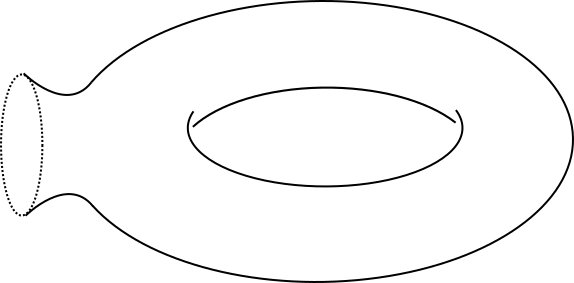
\includegraphics[width=0.5\textwidth]{handle.png}
\caption{A handle.}
\end{figure}

\begin{prop}\label{surface-loops} Let $\Sigma$ be a surface of genus $g$. There exist finite families $R=\{r_i\}$ and $B=\{b_j\}$ of loops on $\Sigma$ such that:
\begin{enumerate}
\item Two loops in the same family are disjoint.
\item Any point of the surface belongs to at most two loops.
\item The loops divide the surface into a disjoint family of regions, each of them a disk (up to homeomorphism).
\end{enumerate}
\end{prop}

\begin{proof} We give an explicit construction of such families.

The case in which $g=0$ (the sphere) is easily dealt with by choosing a single loop $r_1$ as the equator, since both hemispheres are homeomorphic to a disk and the other conditions are vacuously true.

For the cases in which $g>0$, we will make use of the handle decomposition we mentioned previously. We will draw a handle as a square (with opposite edges identified) having a gray hole in its center. Consider the following configuration:

\begin{figure}[h]
\[
\begin{tikzpicture}
\draw (0,0) node[minimum size=6cm,draw] {};

\fill [black,opacity=.15] circle (2cm);

\draw[red] (-3,1) -- (-1.73,1);
\draw[red] (-3,-1) -- (-1.73,-1);

\draw[red] (3,1) -- (1.73,1);
\draw[red] (3,-1) -- (1.73,-1);

\draw[red] (1,-3) -- (1,-1.73);
\draw[red] (-1,-3) -- (-1,-1.73);

\draw[red] (1,3) -- (1,1.73);
\draw[red] (-1,3) -- (-1,1.73);

\draw[blue] (0,0) circle (2cm);
\end{tikzpicture}
\]
\end{figure}

We first deal with the case in which $g=1$. If we glue such a handle to the boundary of the following disk, we obtain a torus with a single red loop $r_1$ and a single blue loop $b_1$:

\begin{figure}[h]
\label{divided-handle}
\[
\begin{tikzpicture}

\draw[red] (-2.83,1) to [bend right=50] (-1,2.83);
\draw[red] (2.83,1) to [bend left=50] (1,2.83);
\draw[red] (2.83,-1) to [bend right=50] (1,-2.83);
\draw[red] (-2.83,-1) to [bend left=50] (-1,-2.83);

\draw[blue] (0,0) circle (3cm);
\end{tikzpicture}
\]
\end{figure}

Once again, the intersection conditions are vacuous. Finally, we observe that the blue loop cuts the torus into a disk and a handle, so one can check condition $3$ in both objects separately. One sees at once that the disk gets cut up into 5 smaller disks, while the handle is divided into $3$ disks, as we wanted.

\marginpar{a lo largo de esta seccion todas las refs a lemas están mal}

While the solution to the case $g=1$ may be easier to draw directly on a square instead of considering a handle decomposition, the latter helps to illustrate the general case, which we now consider. For the case $g>1$, we regard our surface as a disk with $g-1$ holes, with a handle divided as in \ref{divided-handle} attached to its boundary and to each of its holes. We now exemplify the configuration on the \textcolor{red}{holed} disk for $g=4$:

\begin{figure}[h]
\[
\begin{tikzpicture}
\draw[red] (-5.44, 0.5) -- (-3.87, 0.5);
\draw[red] (-5.44, -0.5) -- (-3.87, -0.5);
\draw[red] (5.44, 0.5) -- (3.87, 0.5);
\draw[red] (5.44, -0.5) -- (3.87, -0.5);

\draw[red] (-3.5,0.87) -- (-3.5,2.7);
\draw[red] (-3.5,-0.87) -- (-3.5,-2.7);
\draw[red] (3.5,0.87) -- (3.5,2.7);
\draw[red] (3.5,-0.87) -- (3.5,-2.7);

\draw[red] (-2.137, 0.5) -- (-0.863, 0.5);
\draw[red] (-2.137, -0.5) -- (-0.863, -0.5);
\draw[red] (2.137, 0.5) -- (0.863, 0.5);
\draw[red] (2.137, -0.5) -- (0.863, -0.5);

\draw[red] (-2.5,0.87) to [bend left=40] (-0.5,0.87);
\draw[red] (2.5,0.87) to [bend right=40] (0.5,0.87);
\draw[red] (-2.5,-0.87) to [bend right=40] (-0.5,-0.87);
\draw[red] (2.5,-0.87) to [bend left=40] (0.5,-0.87);

\draw[blue] (0,0) ellipse (5.5cm and 3.5cm);
\draw[blue] (0,0) circle (1cm);
\draw[blue] (-3,0) circle (1cm);
\draw[blue] (3,0) circle (1cm);
\fill [black,opacity=.15] (-3,0) circle (1cm);
\fill [black,opacity=.15] (0,0) circle (1cm);
\fill [black,opacity=.15] (3,0) circle (1cm);
\end{tikzpicture}
\]
\end{figure}

The following is an outline for the construction of the previous figure for general $g$:
\begin{enumerate}
\item Place the $g-1$ holes in a straight line inside the disk.
\item Connect the boundary of the left and rightmost holes to the boundary of the disk using 4 red arcs, mimicking the figure.
\item Cycle through the holes from left to right. If the current hole has a neighboring hole to its right, draw 4 red arcs connecting their boundaries.
\end{enumerate}

Notice that after gluing the handles, both the red and the blue arcs are now loops. We now consider the families $\{r_i\}$ and $\{b_j\}$, consisting of the red and blue loops respectively. Inspecting the figures, we see that conditions 1 and 2 are both satisfied. Finally, it remains to check condition 3. Since we have already seen that each handle is split up into disks in the discussion of the case $g=1$, it suffices to check this for the \textcolor{red}{holed} disk, and once again this is easily seen from the drawing.
\end{proof}


A \emph{band} on a surface $\Sigma$ is a finite sequence $\{C_1, \dots, C_n\}$, where each $S_i$ is a quadrilateral on $\Sigma$ subdivided by one of its main diagonals, arranged as in one of the following two figures:

\[
\begin{tikzpicture}
\draw (-5,1) -- (5,1);
\draw (-5,-1) -- (5,-1);

\foreach \x in {-4,-2,...,4}
\draw (\x,1) -- (\x,-1);

\foreach \x in {-4,-2,...,2}
\draw (\x,-1) -- (\x+2, 1);

\node at (-5,-1.4) {$\dots$};
\node at (-3,-1.4) {$C_{n-1}$};
\node at (-1,-1.4) {$C_{n}$};
\node at (1,-1.4) {$C_{1}$};
\node at (3,-1.4) {$C_{2}$};
\node at (5,-1.4) {$\dots$};
\end{tikzpicture}
\]

\[
\begin{tikzpicture}
\draw (-5,1) -- (5,1);
\draw (-5,-1) -- (5,-1);

\foreach \x in {-4,-2,...,4}
\draw (\x,1) -- (\x,-1);

\foreach \x in {-4,-2,...,2}
\draw (\x,1) -- (\x+2, -1);

\node at (-5,-1.4) {$\dots$};
\node at (-3,-1.4) {$C_{n-1}$};
\node at (-1,-1.4) {$C_{n}$};
\node at (1,-1.4) {$C_{1}$};
\node at (3,-1.4) {$C_{2}$};
\node at (5,-1.4) {$\dots$};
\end{tikzpicture}
\]

Notice that in both cases the choice of diagonal is consistent throughout the band. We will say a band is \emph{positively oriented} if it is arranged as in the first figure and \emph{negatively oriented} otherwise. We require that the only adjacency relations between quadrilaterals in a band are the ones expressed by the figures, so in particular bands have well-defined top and bottom sides. We remark that two differently oriented bands may intersect as the following figure shows:

\[
\label{band-intersection}
\begin{tikzpicture}
\draw (-4,-1) -- (4,-1);
\draw (-4,1) -- (4,1);
\draw (-1,4) -- (-1,-4);
\draw (1,-4) -- (1,4);
\foreach \x in {-3,-1,...,3}
{
\draw (\x,-1) -- (\x, 1);
\draw (-1,\x) -- (1,\x);
}
\foreach \x in {-3,-1,1}
{
\draw (\x,-1) -- (\x+2,1);
\draw (-1,\x) -- (1,\x+2);
}
\end{tikzpicture}
\]

Given a surface $\Sigma$ of arbitrary genus, we consider families of loops $R=\{r_i\}$ and $B=\{b_j\}$ on $\Sigma$ satisfying the conditions stated in proposition \ref{surface-loops}. We can now pick suitably small tubular neighborhoods of each loop and place a positively (resp. negatively) oriented band over each neighborhood corresponding to a loop in $R$ (resp. $B$). Conditions 1 and 2 of proposition \ref{surface-loops} guarantee that all intersections between bands resemble that of figure \ref{band-intersection}. Condition 3 guarantees that each connected component of the complement of the bands is a polygon. We will refer to these polygons as \emph{regions}. Therefore, the collection of bands and regions actually define a polygonal subdivision of $\Sigma$. \textcolor{red}{For technical reasons that will be clearer later, we will require each band to have at least 5 quadrilaterals between any pair of intersections with other bands. This can be easily achieved by refining the division of the band if necessary.} We will refer to this hypothesis as $(\diamond)$ throughout this section. From now on we fix a subdivision as described above for each genus $g$ and call its associated QP $(Q_g,P_g)$. The corresponding Jacobian algebra will be denoted $A_g$.

\begin{figure}[h]
\[
\begin{tikzpicture}
%aristas
\draw (-5, .75) -- (5, .75);
\draw (-5, -.75) -- (5, -.75);
\draw (-5, -5.25) -- (5, -5.25);
\draw (-5, -6.75) -- (5, -6.75);
\draw (-2.25, -8.25) -- (-2.25, 2.25);
\draw (-3.75, -8.25) -- (-3.75, 2.25);
\draw (2.25, -8.25) -- (2.25, 2.25);
\draw (3.75, -8.25) -- (3.75, 2.25);

\foreach \x in {-3.75,-2.25,...,3.75}
{
\draw (\x, .75) -- (\x, -.75);
\draw (\x, -5.25) -- (\x, -6.75);
}

\foreach \x in {-6.75,-5.25,...,1.75}
{
\draw (-3.75, \x) -- (-2.25, \x);
\draw (3.75, \x) -- (2.25, \x);
}

\foreach \x in {-3.75,-2.25,...,2.25}
{
\draw (\x, -.75) -- (\x+1.5, .75);
\draw (\x, -6.75) -- (\x+1.5, -5.25);
}

\foreach \x in {-6.75,-5.25,...,0.25}
{
\draw (-3.75, \x) -- (-2.25, \x+1.5);
\draw (3.75, \x+1.5) -- (2.25, \x);
}

%flechas del quiver
\foreach \x in {-3.75,-2.25,...,2.25}
{
\draw[->, red] (\x+0.85, -0.65) -- (\x+1.4, -0.05);
\draw[->, red] (\x+1.4, 0) -- (\x+0.85, 0);
\draw[->, red] (\x+0.75, -0.1) -- (\x+0.75, -0.65);
\draw[->, red] (\x+0.85, -6.65) -- (\x+1.4, -6.05);
\draw[->, red] (\x+1.4, -6) -- (\x+0.85, -6);
\draw[->, red] (\x+0.75, -6.1) -- (\x+0.75, -6.65);

\draw[->, red] (\x+0.75, 0.1) -- (\x+0.75, 0.65);
\draw[->, red] (\x+0.65, 0.65) -- (\x+0.1, 0.1);
\draw[->, red] (\x+0.1, 0) -- (\x+0.65, 0);
\draw[->, red] (\x+0.75, -5.9) -- (\x+0.75, -5.35);
\draw[->, red] (\x+0.65, -5.35) -- (\x+0.1, -5.9);
\draw[->, red] (\x+0.1, -6) -- (\x+0.65, -6);
}

\foreach \x in {-0.75,-2.25,-3.75}
{
\draw[->, red] (-2.35, \x-0.75) -- (-2.9, \x-0.75);
\draw[->, red] (-3, \x-0.85) -- (-3, \x-1.4);
\draw[->, red] (-2.9, \x-1.4) -- (-2.35, \x-0.85);
\draw[->, red] (3.65, \x-0.75) -- (3.1, \x-0.75);
\draw[->, red] (3, \x-0.85) -- (3, \x-1.4);
\draw[->, red] (3.1, \x-1.4) -- (3.65, \x-0.85);

\draw[->, red] (-3, \x-0.65) -- (-3, \x-0.1);
\draw[->, red] (-3.1, \x-0.1) -- (-3.65, \x-0.65);
\draw[->, red] (-3.65, \x-0.75) -- (-3.1, \x-0.75);
\draw[->, red] (3, \x-0.65) -- (3, \x-0.1);
\draw[->, red] (2.9, \x-0.1) -- (2.35, \x-0.65);
\draw[->, red] (2.35, \x-0.75) -- (2.9, \x-0.75);
}

\draw[<-, red] (-1.4, -0.85) to [bend right] (-0.1, -0.85);
\draw[<-, red] (0.1, -0.85) to [bend right] (1.4, -0.85);
\draw[->,  red] (-1.4, -5.15) to [bend left] (-0.1, -5.15);
\draw[->, red] (0.1, -5.15) to [bend left] (1.4, -5.15);

\draw[->, red] (-2.15, -1.65) to [bend left] (-2.15, -2.9);
\draw[->, red] (-2.15, -3.1) to [bend left] (-2.15, -4.35);
\draw[<-, red] (2.15, -1.65) to [bend right] (2.15, -2.9);
\draw[<-, red] (2.15, -3.1) to [bend right] (2.15, -4.35);

\draw[->, red] (-1.6, -0.85) to [bend left] (-2.15, -1.45);
\draw[->, red] (-2.15, -4.55) to [bend left] (-1.6, -5.15);
\draw[<-, red] (1.6, -0.85) to [bend right] (2.15, -1.45);
\draw[<-, red] (2.15, -4.55) to [bend right] (1.6, -5.15);
\end{tikzpicture}
\]
\caption{The configuration of the associated quiver $Q_g$ around a region.}
\end{figure}
We now turn to the study of some relations that hold in $A_g$, that will enable us to prove its finite-dimensionality.

\begin{lemma}\label{band-sides} Any path in $A_g$ passing through vertices of both sides of a band is zero.
\end{lemma}
\begin{proof} Throughout this and the following proofs, we will only consider our bands to be positively oriented, since the analogous statements for negatively oriented bands are proved in a similar fashion. We name the arrows in the quiver as in the following figure:

\[
\begin{tikzpicture}[text width=1.5mm, font=\footnotesize]
\draw (-5, 0) -- (5, 0);
\draw (-5, 2) -- (5, 2);
\foreach \x in {-3,-1,...,3}
\draw (\x, 0) -- (\x, 2);
\foreach \x in {-3,-1,1}
{
\draw (\x,0) -- (\x+2, 2);
\draw [->, red] (\x+1.9, 1) to node[above] {$b$} (\x+1.1, 1);
\draw[->, red] (\x+1, 0.9) to node[left]{$f$} (\x+1, 0.1);
\draw[->, red] (\x+1.1, 0.1) to node[right]{$a$} (\x+1.9, 0.9);
\draw[->, red] (\x+1, 1.1) to node[right]{$c$} (\x+1, 1.9);
\draw[->, red] (\x+0.9, 1.9) to node[left]{$d$} (\x+0.1, 1.1);
\draw[->, red] (\x+0.1, 1) to node[below]{$e$} (\x+0.9, 1);
}

\draw[->, red, dashed] (-1.9, 2.1) to [bend left] node[above]{$x$} (-0.1, 2.1);
\draw[->, red, dashed] (0.1, 2.1) to [bend left] node[above]{$x$} (2.1, 2.1);
\draw[<-, red, dashed] (-1.9, -0.1) to [bend right] node[below]{$y$} (-0.1, -0.1);
\draw[<-, red, dashed] (0.1, -0.1) to [bend right] node[below]{$y$} (2.1, -0.1);
\end{tikzpicture}
\]

Since our quiver arises from a polygonal subdivision, we know that there is a cycle around each vertex,\marginpar{esto hay que probarlo en algún momento} and so each $x$ and each $y$ are paths of length at least 1. We mark those paths in the figure with a dashed arrow. We have given the same name to arrows occupying the same position in different squares, since this abuse of notation will be useful for calculation.

Inspecting the figure we see that any path passing through vertices of both sides of the band must contain a path of the form $cba$ or $fed$ as factors. It suffices to check that both of them are zero in $A_g$.

We have that $\partial_f(P_g) = ba + eay$, and so $ba  = -eay$ in $A_g$. Therefore, we have that $cba = -ceay$. Moreover, $\partial_d(P_g) = ce + xcb$, from which we deduce that $ce = -xcb$ in $A_g$. Putting all of this together, we get that $cba=-ceay=xcbay$ (one should note that the $cba$ factor in the right hand side of the equality consists of arrows placed on the square immediately left from the one where we started). Proceeding inductively we get $cba=x^ncbay^n$ for all positive $n$. Since $x$ and $y$ are paths of length at least $1$, this shows that $cba$ is equal to paths of arbitrarily high length. Therefore, we conclude that $cba=0$ in $A_g$. \marginpar{esto también hay que hacerlo...}

An analogous argument shows that $fed=0$ in $A_g$ as well, concluding the proof. 
\end{proof}

\begin{lemma}\label{long-band-paths} Any sufficiently long path contained entirely in bands is zero in $A_g$. More precisely, any non-zero path contained in a single band (resp. several bands) is of length at most 5 (resp. 9).
\end{lemma}
\begin{proof} We first prove that any sufficiently long path cotained entirely in a single band is zero. As we have already seen, any path passing through vertices of both sides of the band is zero, so we will suppose without loss of generality that our path is placed on the upper part of the band. Mantaining the notation used on the proof of the previous lemma, this is equivalent to saying our path only has arrows $b, c, d$ or $e$ as factors.

We start by studying paths containing a $3$-cycle as a prefix. The $3$-cycles $edc$ and $ced$ only prefix two paths of length 4, namely $cedc$ and $dced$. Since $\partial_e(P_g) = dc + ayf$, the relation $dc = -ayf$ holds, and so $cedc=-ceayf=0$ and $dced=-ayfed=0$ by lemma \ref{band-sides}. Moreover, the $3$-cycle $dce$ only prefixes two paths of length 5, which are $cbdce$ and $cedce$. Clearly, $cedce=0$ since we have already shown that $cedc=0$, and using the relation $dc=-ayf$ we get $cbdce = - cbayfe=0$ once again by lemma \ref{band-sides}.

Now we turn to paths containing a $3$-cycle as a suffix. Once again, the $3$-cycles $ced$ and $dce$ only suffix two paths of length 4, which are $cedc$ and $dced$, already shown to be zero previously. The $3$-cycle $edc$ is a suffix to only two paths of length 5, which are $edcbd$ and $edced$. We see that $edced=0$ since $dced=0$ and $edcbd=-eayfbd=0$ as we wanted.

Therefore, any path in a band of length $>5$ containing a 3-cycle is zero, since we have shown these cycles only admit prefixes and suffixes of length at most 1.

Now, a path of length $>5$ not containing a 3-cycle is either of the form $dcbdcb$, $bdcbdc$ or $cdbcbd$. All possibilites have $cbdc$ as a factor, which is clearly zero since $cbdc = -cbayf = 0$ by lemma \ref{band-sides}. Therefore, we conclude that any path of length $>5$ contained in a single band is zero.

Finally, consider a path of length $>9$ contained in possibly different bands. If its first six arrows lie on the same band, the path is zero as seen previously. Otherwise, at most five of its first arrows lie on the same band and the sixth is then placed on a different band intersecting the original one, as seen in the following figure:

\[
\begin{tikzpicture}
\draw (-3.5*1.25, 0) -- (1.5*1.25, 0);
\draw (-3.5*1.25, -1.25) -- (1.5*1.25, -1.25);
\draw (0,3.5*1.25) -- (0,-1.5*1.25);
\draw (1.25,3.5*1.25) -- (1.25,-1.5*1.25);

\foreach \x in {-3.75,-2.5,...,0}
{
\draw (\x,-1.25) -- (\x+1.25, 0);
\draw (0, -\x) -- (1.25, -\x);
\draw (\x,0) -- (\x, -1.25);
}

\foreach \x in {0,1.25,...,2.5}
\draw (0, \x) -- (1.25, \x+1.25);

\draw[->, red] (0.5*1.25, 1.5*1.25 - 0.1) -- (0.5*1.25, 1.25 + 0.1);
\draw[->, red] (0.5*1.25 - 0.1, 1.25-0.1) -- (0.1, 0.5*1.25+0.1);
\draw[->, red] (0.1, 0.5*1.25) -- (0.5*1.25 - 0.1, 0.5*1.25);
\draw[->, red] (0.5*1.25, 0.5*1.25-0.1) -- (0.5*1.25, 0.1);
\draw[->, red] (0.5*1.25 - 0.1, -0.1) -- (0.1, -0.5*1.25+0.1);
\draw[->, red] (-0.1, -0.5*1.25) -- (-0.5*1.25+0.1, -0.5*1.25);
\draw[->, red] (-0.5*1.25, -0.5*1.25+0.1) -- (-0.5*1.25, -0.1);
\draw[->, red] (-0.5*1.25 - 0.1, -0.1) -- (-1.25 + 0.1, -0.5*1.25+0.1);
\draw[->, red] (-1.25 -0.1, -0.5*1.25) -- (-1.5*1.25+0.1, -0.5*1.25);
\end{tikzpicture}
\]

Since by hypothesis $(\diamond)$ \marginpar{quizás podria haber un link a la def de $\diamond$}two intersections in the same band are distanced by at least \textcolor{red}{five} quadrilaterals, we conclude that at least the next \textcolor{red}{six} arrows belong to the same band. Therefore, any path of length $>9$ contained entirely in bands is zero in $A_g$, as we wanted.
\end{proof}

\begin{lemma}\label{long-region-paths} Any non-zero path entirely contained in an $n$-sided region is of length at most $3n-4$.
\end{lemma}
\begin{proof} We fix an $n$-sided region. Consider any band neighboring our region and pick any of its squares that is at least two squares away from an intersection with another band, which is always possible by hypothesis $(\diamond)$. Recalling the fact that our region induces an $n$-cycle in the quiver, we name the arrow starting at the square we picked as $x_0$. In general, given $j\in \ZZ/n\ZZ$ we call $x_j$ the arrow starting at the target of $x_{j-1}$. Keeping the previous notation for arrows contained in bands, our current situation is illustrated by this figure:

\[
\begin{tikzpicture}[text width=1.5mm, font=\footnotesize]
\draw (-6, 0) -- (6, 0);
\draw (-6, 2) -- (6, 2);
\foreach \x in {-5,-3,...,5}
\draw (\x, 0) -- (\x, 2);
\foreach \x in {-5,-3,...,3}
{
\draw (\x,0) -- (\x+2, 2);
\draw [->, red] (\x+1.9, 1) to node[above] {$b$} (\x+1.1, 1);
\draw[->, red] (\x+1, 0.9) to node[left]{$f$} (\x+1, 0.1);
\draw[->, red] (\x+1.1, 0.1) to node[right]{$a$} (\x+1.9, 0.9);
\draw[->, red] (\x+1, 1.1) to node[right]{$c$} (\x+1, 1.9);
\draw[->, red] (\x+0.9, 1.9) to node[left]{$d$} (\x+0.1, 1.1);
\draw[->, red] (\x+0.1, 1) to node[below]{$e$} (\x+0.9, 1);
}

\draw[->, red, dashed] (-5+1.1, 2.1) to [bend left] node[above]{$x_{n-2}$} (-5+2.9, 2.1);
\draw[->, red, dashed] (-3+1.1, 2.1) to [bend left] node[above]{$x_{n-1}$} (-3+2.9, 2.1);
\draw[->, red, dashed] (-1+1.1, 2.1) to [bend left] node[above]{$x_{0}$} (-1+2.9, 2.1);
\draw[->, red, dashed] (1+1.1, 2.1) to [bend left] node[above]{$x_{1}$} (1+2.9, 2.1);
\end{tikzpicture}
\]

\marginpar{hay que centrar los labels del dibujo}We now prove that the path $L=x_{n-1}x_{n-2}\dots x_2x_1x_{0}x_{n-1}\dots x_3x_2$ is zero. We have that $\partial_{x_0}(P_g)=x_{n-1}x_{n-2}\dots x_2x_1+cbd$ and $\partial_{x_1}(P_g)=x_{0}x_{n-1}\dots x_3x_2+cbd$. Therefore, the relations
\begin{align*}
x_{n-1}x_{n-2}\dots x_2x_1=-cbd\\
x_{0}x_{n-1}\dots x_3x_2=-cbd
\end{align*}
hold in $A_g$. We stress that $cbd$ denotes a different path in each one of the two equations: they are similar paths contained in different squares. Using this relations, we see that $$ x_{n-1}x_{n-2}\dots x_2x_1x_{0}x_{n-1}\dots x_3x_2=-cbdx_{0}x_{n-1}\dots x_3x_2=cbdcbd,$$ and the latter is zero by lemma \ref{long-band-paths} since $cbdcbd$ is a path of length 6 lying on a single band. 

Finally, since the longest path entirely contained in our region not having $L$ as a factor is
$$x_{n-2}x_{n-1}\dots x_0x_{n-1}x_{n-2}\dots x_0x_{n-1}x_{n-2}\dots x_3,$$
\marginpar{poner las longitudes con ganchitos}which is of length $3n-4$, the result follows.
\end{proof}

\begin{lemma} \label{long-br-paths} Any sufficiently long path not having factors from two different regions is zero in $A_g$.
\end{lemma}
\begin{proof} We write our path as $B_{k+1}R_k\dots R_2 B_2 R_1 B_1$, where the paths $R_i$ are contained in a same region and the paths $B_j$ are non-trivial (except possibly for $B_1$ and $B_{k+1}$) and contained in bands.

Let $1<j<k+1$. The path $B_j$ starts and ends at the boundary of our region of interest. Therefore, it must pass through both of the endpoints of a same arrow belonging to the cycle associated to the region, which we will call $x_0$ following the notation employed in the proof of lemma \label{long-band-paths}.\marginpar{esto no está particularmente claro...} Therefore, using the relation induced by $\partial_{x_0}(P_g)$, we can replace some of the arrows in $B_j$ with a path entirely contained in the region.
After applying this argument repeatedly, we can then suppose our path is of the form $B_2 R_1 B_1$. The proof now follows from lemmas \ref{long-band-paths} and \ref{long-region-paths}, since if our path is non-zero, then $|B_1|<10$, $|B_2|<10$ and $|R_1|<3n-3$, where $n$ is the number of sides of the region.
\end{proof}

After proving all these lemmas, the main result of this section now easily follows:

\begin{thm} The algebra $A_g$ is finite-dimensional.
\end{thm}
\begin{proof} By lemma \ref{long-br-paths}, any sufficiently long path is zero if it does not have factors from two different regions, but any path that does must be zero (regardless of length) by lemma \ref{band-sides}, since it must cross a band. Therefore, any sufficiently long path is zero, and so $A_g$ is finite-dimensional.
\end{proof}
\end{section}
\end{chapter}
\begin{chapter}{Cohomological properties}
In the previous chapter, we produced confluent rewriting systems for several Jacobian algebras. As we have noted, such a rewriting system provides a basis for the algebra as a $k$-vector space, which is given by the irreducible monomials. In this chapter, we will make use of these bases to compute some invariants of the families of algebras considered previously. These invariants are closely related to the first two Hochschild cohomology modules of those algebras, which we will now introduce.

Given an associative $k$-algebra $A$, we define its \emph{enveloping algebra} as $A^e=A\otimes_k A^{\mathrm{opp}}$. The product on $A^e$ is given by $(a\otimes b)(c\otimes d)=ac\otimes db$.
There is a natural equivalence between the category of $A$-$A$-bimodules and the category of left $A^e$-modules, which we will consider an identification. Therefore, if $M$ is an $A$-$A$-bimodule, it makes sense to compute $\Ext^\bullet_{A^e}(A,M)$, which we will call the \emph{Hochschild cohomology of $A$ with coefficients in $M$} and denote $H^\bullet(A,M)$.
If $M=A$, this module will be plainly called the \emph{Hochschild cohomology of $A$}, and will be denoted as $HH^\bullet(A)$.

\begin{section}{The center}
Let $A$ be an associative $k$-algebra. The \emph{center} of $A$, denoted as $\mathcal{Z}(A)$, is the subset of all elements $x\in A$ such that $xa=ax$ for all $a\in A$, and is in fact a subalgebra of $A$. An algebra is called \emph{central} if $\mathcal{Z}(A)=k$. For example, the matrix algebra $M_n(k)$ is a central $k$-algebra.

\begin{lemma} Let $A$ be an associative $k$-algebra. Then $HH^0(A) = \mathcal{Z}(A)$.
\end{lemma}
\begin{proof} See \cite{Red01}.
\end{proof}

We will now compute the center of the Jacobian algebras associated to pyramids, prisms and antiprisms. In order todo so, we first make a useful observation:

\begin{obs}\label{central-endpoints} Let $x$ be a central element in a Jacobian algebra $A$. Then $x$ is a linear combination of \emph{loops}, that is, paths with identical source and target.
\end{obs}
\begin{proof} First of all, we stress that two paths which are equivalent in the Jacobian algebra must share the same endpoints, since the Jacobian ideal is generated by sums of paths satisfying this property. Therefore, it makes sense to speak of endpoints and loops in $A$.

Suppose now that $x$ is central in $A$. We write $x$ as a combination of linearly independent classes of paths $\sum_{i=1}^n \lambda_i p_i$. Let $v_j$ be the stationary path corresponding to the source of $p_j$. Since $x$ is central, we have that
\[\sum_{i=1}^n \lambda_i p_iv_j=(\sum_{i=1}^n \lambda_i p_i)v_j = xv_j=v_jx = v_j(\sum_{i=1}^n \lambda_i p_i)=\sum_{i=1}^n \lambda_i v_jp_i.\]
The scalar corresponding to $p_j$ in the left hand side of the equation is $\lambda_j$, since $p_jv_j=p_j$. However, the scalar corresponding to $p_j$ on the right hand side is $\lambda_j$ if $p_j$ has the vertex at $v_j$ as target, and 0 otherwise. Therefore, if $p_j$ is not a loop, then $\lambda_j=0$, and so $x$ is a linear combination of loops, as we wanted.
\end{proof}

We remark that, by definition, stationary paths are loops. Moreover, it is easy to see that any loop commutes with all stationary paths.

As a consequence of the diamond lemma, we know that given a confluent rewriting system for a Jacobian algebra, the set of irreducible monomials forms a basis for it. This will be an essential tool to compute its center. In what follows, we will maintain the notation for paths used in the previous chapter.

\begin{prop} The Jacobian algebra associated to a pyramid with $n$-sided base, where $n>3$, is central.
\end{prop}
\begin{proof} Suppose first that $n$ is even. The confluent rewriting system found previously induces the basis of irreducible paths 
\[B=\{e_v,a^k,b^k,cb^j, da^j\},\] 
where $v$ runs through the set of vertices $Q_0$, $1\leq k\leq 2n-3$ and $0\leq j\leq n-2$.\note{modificar el texto de las derivaciones para que no quede tan redundante} Notice that the label $a^k$ denotes $n$ different cycles, each starting at a different vertex. We will enumerate those vertices from $0$ to $n-1$, in such a way that if $i+1=j \mod n$ then there exists an $a$ arrow starting at vertex $i$ and ending at vertex $j$. We will denote the path starting at vertex $k$ consisting of $j$ arrows labeled $a$ as $a_k^j$. For example, using this notation, we have that $a_1a_0=a_0^2$. Notice that $a_k^n$ both starts and ends at $k$, since it is a cycle. We will use the same idea to name the $n$ different cycles of the form $b^n$.

Now, the only irreducible loops are of the form $e_v$, $a^n$ or $b^n$, and so if we write a central element $x$ in terms of our basis $B$, by \hyperref[central-endpoints]{Observation \ref*{central-endpoints}} we get that
\[x = \sum_{v\in Q_0} \lambda_v e_v + \sum_{i\in \ZZ/n\ZZ}(\mu_i a_i^n + \eta_i b_i^n),\]
where all greek letters are scalars. Since $x$ is central, it must commute with $a_i$, and so:
\[\lambda_{s(a_i)}a_i + \mu_{i-1} a_{i-1}^{n+1}=a_ix = xa_i = \lambda_{t(a_i)}a_i + \mu_{i+1} a_i^{n+1}.\]
Exactly the same identity holds if we replace $a_i$ with $b_i$ throughout. Running down through all possible values of $i$, this set of equalities imply that all $\mu$ (resp. $\eta$) scalars are zero and that $\lambda_u=\lambda_v$ if $u$ and $v$ are vertices which are sources of $a$ (resp. $b$) arrows.

We now observe that every vertex of the quiver is either the source of an $a$ or a $b$ arrow. Therefore $x=\lambda_1 y + \lambda_2 z$, where $y$ (resp. $z$) denotes the sum of all stationary paths corresponding to vertices which are sources of $a$ (resp. $b$) arrows. Now, since $x$ is central, it must commute with any $c$ arrow, and thus
\[\lambda_2 c = cx = xc = \lambda_1 c,\]
from where we obtain $\lambda_1=\lambda_2$. Therefore, any central element must be a scalar multiple of the sum of all stationary paths, which is the identity element of the algebra. Thus, we conclude that the Jacobian algebra is central, as we wanted.

The case where $n$ is odd is entirely analogous. The only minor difficulty is that cycles of different lengths appear in the generic expression of a central element, since cycles of the form $a^{kn}$ or $b^{kn}$ are irreducible even if $k>1$. Nevertheless, the only difference this introduces is that the equations we used are somewhat more cumbersome to write down.
\end{proof}

\begin{prop} Let $A$ be the Jacobian algebra associated to a prism with $n$-sided base, where $n>3$. Then, $\mathcal{Z}(A) = \langle 1, a^n, b^n, edcf\rangle$, where 1 stands for the identity element of $A$.
\end{prop}
\begin{proof} First of all, we notice that any cycle $x$ of the form $a^n$, $b^n$ or $edcf$ is central. Indeed, they commute with stationary paths since they are loops, and if $y$ is a path of positive length then the rewriting system shows that $yx=xy=0$.

Since the only irreducible loops are either stationary or of the form $a^n$, $b^n$ or $edcf$, an arbitrary central element $x$ can be written down as 
\[x = \sum_{v\in Q_0} \lambda_v e_v + y,\]
where $y\in \langle a^n,b^n, edcf\rangle$ and is thus central. Considering that $\mathcal{Z}(A)$ is a subspace and both $x$ and $y$ are central, we get that $x-y=\sum_{v\in Q_0} \lambda_v e_v$ is as well. Now, let $p$ be any arrow in the quiver. Then, by centrality we have that
\[\lambda_{s(p)}p= p\sum_{v\in Q_0} \lambda_v e_v=\sum_{v\in Q_0} \lambda_v e_vp = \lambda_{t(p)}p,\]
and so $\lambda_{s(p)}=\lambda_{t(p)}$. But then, since the quiver is strongly connected, an easy induction on the distance between any pair of paths shows that $\lambda_u=\lambda_v$ for all $u,v\in Q_0$. Thus, $x= \lambda 1 +y$, proving our claim.
\end{proof}

\begin{prop} Let $A$ be the Jacobian algebra associated to an antiprism with $n$-sided base, where $n>3$. Then, $\mathcal{Z}(A) = \langle 1, egaf, dbch\rangle$, where 1 stands for the identity element of $A$.
\end{prop}
\begin{proof} We will only sketch the proof, since it uses the same arguments as the previous two propositions. The loops $egaf$ and $dbch$ are easily seen to be central, because any product involving them and a path of positive length is zero, just as what happened in the proof of the previous proposition.

Now, in this case, the irreducible loops are stationary or of the form $a^n$, $b^n$, $egaf$ or $dbch$. Thus, a generic central element $x$ is of the form
\[x = \sum_{v\in Q_0} \lambda_v e_v + y + z,\]
where $y\in\langle a^n, b^n\rangle$ and $z\in\langle egaf, dbch\rangle\subseteq \mathcal{Z}(A)$. Using the same argument as in the pyramidal case, namely multiplying by $a$, $b$ on the left and right, we see that $y=0$.

Since $x$ and $z$ is central, so is $x-z= \sum_{v\in Q_0} \lambda_v e_v$, and once again a connection argument shows that $x-z$ must be a scalar multiple of the identity. Therefore, $x=\lambda 1 + z$, as we wanted.
\end{proof}
\end{section}

\begin{section}{Derivations}
Let $A$ be a $k$-algebra. A \emph{derivation} of $A$ is a $k$-linear morphism $f:A\to A$ satisfying the \emph{Leibniz rule}
\[f(ab)=f(a)b+af(b).\]
The set of derivations of $A$, which we will denote as $D(A)$, is a Lie algebra with Lie bracket given by the commutator
\[[f,g] = f\circ g - g\circ f.\]
If $x\in A$, the map $f_x(y) = xy-yx$ is a derivation. The set of such maps, which we call \emph{inner derivations}, is denoted $\Inn(A)$, and it is actually a $k$-subspace of $D(A)$. Our main interest in derivations relies on the following fact:

\begin{lemma} Let $A$ be an associative $k$-algebra. Then $HH^1(A) = D(A)/\Inn(A)$.
\end{lemma}
\begin{proof} See \cite{Red01}.
\end{proof}

Recall that, given a quiver $Q$, we denote its vertex span $k^{Q_0}$ as $R$. Since a Jacobian algebra $A$ is an $R$-bimodule, it makes sense to consider the Lie subalgebra of $R$-linear derivations of $A$, which we will denote $D_R(A)$. The following easy observations will greatly simplify our work:
\begin{obs}\label{derivation-quotient} Let $A$ be a $k$-algebra and $I\subseteq A$ an ideal. If $f$ is a derivation of $A$ such that $f(I)\subseteq I$, then the induced linear map $\hat{f}:A/I\to A/I$ is a derivation of $A/I$. Moreover, if $R$ is a set of generators for $I$, it suffices to see that $f(R)\subseteq I$ to show that $f(I)\subseteq I$.
\end{obs}
\begin{proof} Since $f(I)\subseteq I$, the ideal $I$ is contained in the kernel of $\pi\circ f:A\to A/I$, where $\pi$ denotes the natural projection. Thus there is a well defined linear map $\hat{f}:A/I\to A/I$ which obviously satisfies the Leibniz rule, since $f$ does.

As for the second assertion, suppose $x\in I$. Then $x=\sum_{i=1}^n a_ir_ib_i$, where $r_i\in R$ and $a_i, b_j\in A$. Therefore, the Leibniz rule implies that
\[f(x) = \sum_{i=1}^n f(a_ir_ib_i)=\sum_{i=1}^n \left(f(a_i)r_ib_i + a_if(r_i)b_i + a_ir_if(b_i)\right)\in I\]
since by hypothesis $f(R)\subseteq I$.
\end{proof}
\begin{obs}\label{derivation-vertices} Let $v\in R$ be a stationary path in a Jacobian algebra $A$. If $f$ is an $R$-linear derivation of $A$, then $f(v)=0$.
\end{obs}
\begin{proof} Using the Leibniz rule, the $R$-linearity of $f$ and the fact that $v=v^2$, we have that
\[f(v)= f(v^2)= f(v)v + vf(v)=f(v^2)+ f(v^2)=2f(v^2)=2f(v)\]
and so $f(v)=0$.
\end{proof}
\begin{obs}\label{endpoints} Let $B$ be a path basis for a Jacobian algebra $A$. If $f$ is an $R$-linear derivation of $A$ and $p\in B$, then $f(p)$ is a linear combination of elements of $B$ only involving paths sharing the same endpoints as $p$.
\end{obs}
\begin{proof} Since $B$ is a basis for $A$, we have that
\[f(p) = \sum_{q\in B} \lambda_q q\]
for some scalars $\lambda_q\in k$. Let $x, y\in R$ be the source and the target of $p$, respectively. Then
\[\sum_{q\in B} \lambda_q q=f(p)=f(ypx) = yf(p)x =\sum_{q\in B} \lambda_q yqx,\]
and so $\lambda_q=0$ if $q$ has different endpoints than $p$.
\end{proof}
From now on, we will refer to $R$-linear derivations plainly as derivations. We will also maintain the labeling of arrows presented in the previous chapter for the quivers associated to each polygonal subdivision.

\begin{subsection}{Pyramids with an even-sided base}
Let $n$ be an even number greater than 3. In \hyperref[pyramids]{Section \ref*{pyramids}}, we proved that the Jacobian algebra $A$ associated with a pyramid having an $n$-sided base is finite-dimensional. Following the notation used in that section, a basis of irreducible monomials for the rewriting system we found is given by
\[B=\{e_v,a^k,b^k,cb^j, da^j\},\] 
where $v$ runs through the set of vertices $Q_0$, $1\leq k\leq 2n-3$ and $0\leq j\leq n-2$. Once again, we are abusing notation, since for instance $a$ denotes several different paths of length 1. For simplicity, we will only study derivations $f$ that assign the same value to all paths sharing the same name. Thus, we may speak of the value of $f(a)$ in an unambigous manner.

If $f$ is such a derivation of $A$, then by \hyperref[endpoints]{Observation \ref*{endpoints}} we have that
\begin{equation}
\begin{aligned}
\label{pyramid-equations}
f(a) &= \alpha a + \hat\alpha a^{n+1}\\
f(b) &= \beta b + \hat\beta b^{n+1}\\
f(c) &= \gamma c \\
f(d) &= \delta d,
\end{aligned}
\end{equation}
where all greek letters are scalars in $k$. We recall that the following relations generate the Jacobian ideal $I$:
\begin{align}
a^{n+1}+cd \label{eq-a}\\
b^{n+1}+dc \label{eq-b}\\
bd+da \label{eq-c}\\
ac+cb \label{eq-d}
\end{align}
By relation \eqref{eq-a} and the Leibniz rule, we have that
\begin{align*}-(\gamma+\delta)cd&= -f(c)d - cf(d)\\
&= f(-cd)\\
&=f(a^{n+1})\\
&=\sum_{m=0}^{n} a^mf(a)a^{n-m}\\
&=\sum_{m=0}^{n} a^m(\alpha a + \hat\alpha a^{n+1}) a^{n-m}\\
&=(n+1)(\alpha a^{n+1} + \hat\alpha a^{2n+2})\\
&=(n+1)\alpha a^{n+1}\\
&=-(n+1)\alpha cd,
\end{align*}
and so $\gamma+\delta = (n+1)\alpha$. Reasoning analogously using relation \eqref{eq-b}, we conclude that $\gamma+\delta = (n+1)\beta$, and thus $\alpha=\beta$.

Relation \eqref{eq-c} implies
\begin{align*}-(\beta+\delta)bd &=-(\beta+\delta)bd - \hat\beta bd^{n+1}\\
&=-f(b)d - bf(d)\\
&=f(-bd)\\
&=f(da)\\
&=f(d)a+df(a)\\
&=(\delta+\alpha)da + \hat\alpha da^{n+1}\\
&=(\delta+\alpha)da\\
&=-(\delta+\alpha)bd,
\end{align*}
and thus we get the equation $\alpha=\beta$ again. Relation \eqref{eq-d} implies the same identity as well.

Now, if $g$ is a derivation of $\kQ$ satisfying the set of equations \eqref{pyramid-equations}, its values on $a,b,c$ and $d$ completely determine it, since any path is either a stationary path (which is mapped to zero by \hyperref[derivation-vertices]{Observation \ref*{derivation-vertices}}) or equal to a unique product of $a,b,c$ and $d$, and thus its image is uniquely determined by the Leibniz rule. Moreover, as we have just seen, if $\alpha=\beta$ and $\gamma+\delta=(n+1)\alpha$ then the image of a set of generators of $I$ by $g$ is contained in $I$, and so $g$ induces a derivation of the Jacobian algebra \note{decir por qué esta bien hacerlo desde el álgebra sin completar} by \hyperref[derivation-quotient]{Observation \ref*{derivation-quotient}}.

We now write the values of a generic derivation of the form we described in terms of the basis $B$:
\begin{align*}
g(e_v) &= 0\\
g(a^k) &=\sum_{m=0}^{k-1} a^mg(a)a^{k-1-m}=k(\alpha a^k + \hat\alpha a^{n+k}) \\
g(b^k) &=\sum_{m=0}^{k-1}b^mg(b)b^{k-1-m}=k(\alpha b^k + \hat\beta b^{n+k})\\
g(cb^j) &= g(c)b^j + cg(b^j) = (\gamma+j\alpha) cb^j \\
g(da^j) &= g(d)a^j + dg(a^j) = (\delta+j\alpha) da^j = \left((n+j+1)\alpha-\gamma\right)da^j
\end{align*}
It is clear that these derivations make up a vector space $V$ of dimension 4. A basis for this space is given by $\{\alpha^*, \gamma^*, \hat\alpha^*, \hat\beta^*\}$, where $\alpha^*$ stands for the map defined by setting $\alpha=1$ and $\hat\alpha=\beta=\gamma=0$, and the other maps are defined analogously. We now write down the image of the basis $B$ in terms of these maps to ease computation:
\begin{center}
\begin{tabular}{ c | c | c | c | c }
	& 	$\alpha^*$ 		& $\gamma^*$	& $\hat\alpha^*$	& $\hat\beta^*$	\\
\hline
$e_v$ & 	0 			& 0 			& 0			& 0 \\
$a^k$ & 	$ka^k$ 		& 0			& $ka^{n+k}$	& 0 \\
$b^k$ & 	$kb^k$ 		& 0			& 0			& $kb^{n+k}$ \\
$cb^j$ & 	$jcb^j$ 		& $cb^j$		& 0			& 0 \\
$da^j$ & 	$(n+j+1)da^j$	& $-da^j$		& 0			& 0 
\end{tabular}
\end{center}

From this table we see that $B$ is a basis of eigenvectors for both $\alpha^*$ and $\gamma^*$, and thus these two maps commute. Moreover, $\gamma^*$, $\hat\alpha^*$ and $\hat\beta^*$ commute with each other as well, since they act trivially outside of $\langle cb^j, da^j\rangle$, $\langle a^k\rangle$ and $\langle b^k\rangle$ respectively, and these three spaces are in direct sum. These facts imply the vanishing of the brackets $[\alpha^*,\gamma^*]$,  $[\gamma^*, \hat\alpha^*]$, $[\gamma^*, \hat\beta^*]$ and $[\hat\alpha^*, \hat\beta^*]$. By direct computation \note{explicitar la cuenta?} using the table we see that $[\alpha^*,\hat\alpha^*]=n\hat\alpha^*$ and $[\alpha^*,\hat\beta^*]=n\hat\beta^*$. Therefore, $V$ is actually closed under the Lie bracket and so is a 4-dimensional Lie subalgebra of the algebra of derivations of $A$.

In fact, we may further characterize the Lie structure on $V$. Given Lie algebras $L_1$ and $L_2$ and an action by derivations $\cdot$ of $L_1$ on $L_2$, the \emph{semi-direct product $L_1\ltimes L_2$} is the $k$-vector space $L_1 \oplus L_2$ with Lie bracket given by
\[[(x_1,x_2), (y_1,y_2)] = ([x_1,y_1], [x_2,y_2]+x_1\cdot y_2 - y_1\cdot x_2).\]
It is now easy to see that $V$ is a semi-direct product of the abelian Lie algebras $\langle \alpha^*\rangle$ and $\langle \gamma^*, \hat\alpha^*, \hat\beta^*\rangle$, where $\alpha^*$ acts trivially over $\gamma^*$ and by multiplication by $n$ over $\hat\alpha^*$ and $\hat\beta^*$.
\end{subsection}

Following the exact same modus operandi, we will now produce non-trivial derivations for the Jacobian algebras arising from prisms and antiprisms. Since in these cases there are more relations generating the Jacobian ideal than in the pyramidal case, the derivations will have to satisfy more constraints.

\begin{subsection}{Prisms}
As in the previous subsection, any derivation $\psi$ of the Jacobian algebra $A$ associated to a prism with an $n$-sided base must send paths to paths sharing the same endpoints. Therefore, by writing the image of the paths of length 1 by $\psi$ in the basis of irreducible monomials, we find that $\psi$ must satisfy:
\begin{align*}
\psi(a) &= \alpha a\\
\psi(b) &= \beta b\\
\psi(c) &= \gamma c \\
\psi(d) &= \delta d \\
\psi(e) &= \varepsilon e \\
\psi(f) &= \zeta f
\end{align*}
Notice that in this case there are no pairs of different paths sharing the same endpoints, which will make the rest of the computation quite easier. Mimicking the process carried out in the pyramidal case, we obtain constraints (in the right column) for the greek scalars using the relations that span the Jacobian ideal (in the left column) and the Leibniz rule:
\begin{align*}
de+a^{n-1} &  	&\delta+\varepsilon 	&=(n-1)\alpha\\
fc+b^{n-1}  &  	&\zeta+\gamma 		&=(n-1)\beta\\
ad+dcf	&	&\alpha+\delta		&=\delta+\gamma+\zeta\\
bf+fed	&	&\beta+\zeta		&=\zeta+\varepsilon+\delta\\
ea+cfe	&	&\varepsilon+\alpha	&=\gamma+\zeta+\varepsilon\\
cb+edc	&	&\gamma+\beta		&=\varepsilon+\delta+\gamma
\end{align*} 
Solving the linear system of equations on the right column, we find that $\alpha=\beta=0$, $\delta=-\varepsilon$ and $\gamma=-\zeta$. Once again, any set of scalars satisfying these constraints induces a derivation of the path algebra that passes to the quotient and induces a bonafide derivation of $A$. We thus obtain two linearly independent derivations of $A$, $\gamma^*$ and $\delta^*$, which are defined on paths of length 1 as
\begin{center}
\begin{tabular}{ c | c | c }
	& 	$\gamma^*$ 	& $\delta^*$\\
\hline
$a$ & 0 		& 0		\\
$b$ & 	0 		& 0		 \\
$c$ & 	$c$ 		& 0	 \\
$d$ & 	0		& $d$	\\
$e$ & 0		& $-e$ \\
$f$ & $-f$		& 0
\end{tabular}
\end{center}
\end{subsection}
\begin{subsection}{Antiprisms}
We follow the usual drill, this time for antiprisms. We start by writing down the image of the paths of length 1 by an eventual derivation $\psi$ in the basis of irreducible monomials, and find that $\psi$ must satisfy:
\begin{align*}
\psi(a) &= \alpha a +\hat\alpha a^{n+1}\\
\psi(b) &= \beta b + \hat\beta b^{n+1}\\
\psi(c) &= \gamma c \\
\psi(d) &= \delta d \\
\psi(e) &= \varepsilon e \\
\psi(f) &= \zeta f \\
\psi(g) &= \eta g \\
\psi(h) &= \theta h
\end{align*}
Once again, we have two pairs of paths sharing the same endpoints. We now find the constraints the scalars must verify using the relations in the Jacobian ideal:
\begin{align*}
feg+a^{n-1} &  	&\zeta+\varepsilon+\gamma 	&=(n-1)\alpha\\
chd+b^{n-1}  &  	&\gamma+\theta+\delta 		&=(n-1)\beta\\
ed+hbd	&	&\varepsilon+\delta		&=\theta+\beta+\delta\\
ce+bch	&	&\gamma+\varepsilon		&=\beta+\gamma+\theta\\
dc+gaf	&	&\delta+\gamma			&=\eta+\alpha+\zeta\\
hg+ega	&	&\theta+\eta			&=\varepsilon+\eta+\alpha\\
fh+afe	&	&\zeta+\theta			&=\alpha+\zeta+\varepsilon\\
gf+dbc	&	&\eta+\zeta				&=\delta+\beta+\gamma
\end{align*} 
The linear system of equations on the right column imposes the following constraints:
\begin{align*}
\alpha=\beta=0\\
\delta=-\gamma-\varepsilon\\
\eta=-\varepsilon-\zeta\\
\theta=-\varepsilon
\end{align*}
Any solution for this system of equations induces a derivation of the Jacobian algebra of the antiprism in the usual manner. We thus obtain five linearly independent derivations: $\hat\alpha^*$, $\hat\beta^*$, $\gamma^*$, $\varepsilon^*$ and $\zeta^*$, which values on the set of paths of length 1 we present on the following table:
\begin{center}
\begin{tabular}{ c | c | c | c | c | c }
	& $\hat\alpha^*$ 		& $\hat\beta^*$	& $\gamma^*$	& $\varepsilon^*$	& $\zeta^*$\\
\hline
$a$ & 	$a^{n+1}$ 			& 0			& 0			& 0 			& 0 \\
$b$ & 	0 				& $b^{n+1}$	& 0			& 0 			& 0 \\
$c$ & 	0 				& 0			& $c$			& 0 			& 0 \\
$d$ & 	0				& 0			& $-d$		& $-d$ 		& 0 \\ 
$e$ & 	0				& 0			& 0			& $e$ 			& 0 \\
$f$ & 	0				& 0			& 0			& 0 			& $f$ \\
$g$ & 	0				& 0			& 0			& $-g$		& $-f$ \\
$h$ & 	0				& 0			& 0			& $-h$		& 0 
\end{tabular}
\end{center}
\end{subsection}
\end{section}
\end{chapter}
\begin{appendix}
\begin{chapter}{A path algebra SageMath class}
\label{appendix}
We have developed a \texttt{SageMath} class to deal with the long and tedious process of checking the hypotheses of the diamond lemma, and to automatically generate bases and compute some invariants of the Jacobian algebra associated to a polygonal subdivision, with the only input being the subdivision itself. We now present the source code, which we will then discuss in more detail:
\lstinputlisting{rewsystems.py}
We will explain how the program works by following an example execution in which we will compute some invariants of pyramids, as studied in \hyperref[pyramids]{Section \ref*{pyramids}}.

An instance of the \texttt{Rewriting\_System} class is constructed from an undirected graph representing a polygonal subdivison of the sphere. The associated quiver and standard potential will be automatically generated. We only implemented this feature for the spherical case since an enumeration of the faces of the polygonal subdivision is carried out by finding a planar embedding of the graph on the surface, and \texttt{SageMath} only provides such an algorithm for the sphere.

We would like to generate the rewriting system associated to a pyramid with an odd-sided base. In order to do that, we use the following snippet, which produces a pyramid with an $n$-sided base:
\begin{lstlisting}
def pyramid(n):
  edges = {}
  for i in xrange(1, n):
    edges[i] = [i+1, n+1]
  edges[n] = [1, n+1]
  return Graph(edges)
\end{lstlisting}
We now instantiate our desired triangulation:
\begin{lstlisting}
sage: odd_pyramid = pyramid(5)
sage: odd_pyramid.show()
\end{lstlisting}
\begin{figure}[h]
\centering
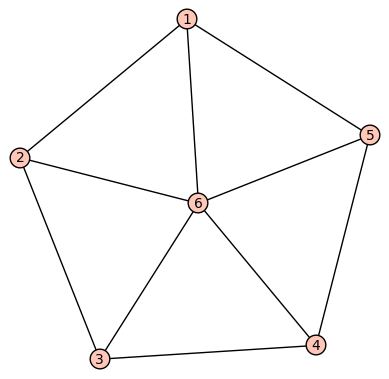
\includegraphics[width=0.5\textwidth]{odd_pyramid.png}
\end{figure}
Before producing the rewriting system, let us explain how the class constructor works. As mentioned previously, the QP will be automatically generated. If the \texttt{zero\_rules\_flag} is set to \texttt{False}, the \texttt{rewriting\_rules()} method will produce the set of usual rewriting rules (the ones associated to the revglex order) and perform \hyperref[heuristic]{Heuristic \ref*{heuristic}} indefinitely until confluence is achieved. In order to test confluence, for every ambiguity we reduce both of its branches a maximum of \texttt{ambiguity\_depth} times and compare if both branches eventually resolve to the same element.

If the \texttt{zero\_rules\_flag} is set to \texttt{True}, the following heuristic will be executed just after producing the first set of rewriting rules, which are the ones that arise from the Jacobian relations:
\begin{heur} As we have seen in \hyperref[arbitrarily-long]{Observation \ref*{arbitrarily-long}},  any path that may be prolonged to a path of arbitrarily high length is zero. Reductions of the form $x\rightsquigarrow 0$ are highly desirable, since the ambiguities they generate are usually simple to resolve. Obviously, if $x=0$, then $yxz=0$ for all $y,z$, and so we are interested in finding only the shortest paths that reduce to zero. Therefore, we perform the following steps:
\begin{enumerate}
\item Let $n=2$.
\item Produce a list of all paths of length $n$.
\item Apply rewriting rules to each path until either they are irreducible or they are longer than \texttt{zero\_depth}.
\item If a path $x$ is equal to a path of length greater than \texttt{zero\_depth}, add the rewriting rule $x\rightsquigarrow 0$.
\item If no path was found to reduce to zero, increase $n$ by 1 and repeat steps 2 to 5.
\end{enumerate}
This may be formalized by a \textcolor{red}{pumping lemma argument} if we choose a high enough value for \texttt{zero\_depth}.
\end{heur}

We now generate the rewriting system associated to our pyramid:
\begin{lstlisting}
sage: odd_rs = Rewriting_System(odd_pyramid)
9 rules added.
4 rules added.
Total rules: 33
\end{lstlisting}
As we can see, the program had to enlarge the set of rules twice before achieving confluence. Let us examine the quiver and its associated potential, which both were generated automatically out of the triangulation:
\begin{lstlisting}
sage: odd_rs.quiver.show()
\end{lstlisting}
\begin{figure}[h]
\centering
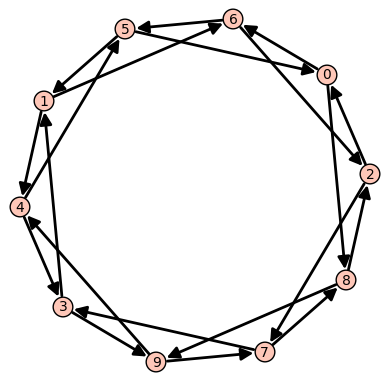
\includegraphics[width=0.5\textwidth]{odd_quiver.png}
\end{figure}
\begin{lstlisting}
sage: odd_rs.potential
[[8, 5, 6, 8],
 [3, 4, 6, 3],
 [0, 3, 5, 7, 1, 0],
 [7, 8, 9, 7],
 [1, 9, 2, 1],
 [4, 0, 2, 4],
 [0, 2, 1, 0],
 [0, 3, 4, 0],
 [3, 5, 6, 3],
 [5, 7, 8, 5],
 [1, 9, 7, 1],
 [2, 4, 6, 8, 9, 2]]
\end{lstlisting}
As the output shows, there are five 3-cycles coming from the triangular faces, a 5-cycle from the pentagonal face, five 3-cycles from punctures where three faces meet and another 5-cycle from the puncture corresponding to the apex of the pyramid.

The confluent rewriting system found by the software is given by this set of 33 rules:
\begin{lstlisting}
sage: odd_rs.rules
{(0, 2, 1): -(0, 3, 5, 7, 1),
 (0, 2, 4): -(0, 3, 4),
 (1, 0, 2): -(1, 9, 2),
 (1, 0, 3, 4): (1, 9, 2, 4),
 (1, 0, 3, 5, 6): -(1, 9, 2, 4, 6),
 (1, 0, 3, 5, 7, 8): (1, 9, 2, 4, 6, 8),
 (1, 9, 2, 4, 6, 8, 9, 7): (1, 0, 3, 5, 7, 1, 0, 3, 5, 7),
 (1, 9, 7): -(1, 0, 3, 5, 7),
 (2, 1, 0): -(2, 4, 0),
 (2, 1, 9): -(2, 4, 6, 8, 9),
 (3, 4, 0): -(3, 5, 7, 1, 0),
 (3, 4, 6): -(3, 5, 6),
 (4, 0, 2): -(4, 6, 8, 9, 2),
 (4, 0, 3): -(4, 6, 3),
 (5, 6, 3): -(5, 7, 1, 0, 3),
 (5, 6, 8): -(5, 7, 8),
 (5, 7, 1, 0, 3, 4): -(5, 7, 8, 9, 2, 4),
 (6, 3, 4): -(6, 8, 9, 2, 4),
 (6, 3, 5): -(6, 8, 5),
 (6, 8, 9, 2, 4, 0): (6, 8, 9, 7, 1, 0),
 (7, 1, 0, 3, 5, 6): (7, 8, 9, 2, 4, 6),
 (7, 1, 9): -(7, 8, 9),
 (7, 8, 5): -(7, 1, 0, 3, 5),
 (7, 8, 9, 7): (7, 1, 0, 3, 5, 7),
 (8, 5, 6): -(8, 9, 2, 4, 6),
 (8, 5, 7): -(8, 9, 7),
 (8, 9, 2, 4, 6, 3): -(8, 9, 7, 1, 0, 3),
 (9, 2, 1): -(9, 7, 1),
 (9, 2, 4, 0): (9, 7, 1, 0),
 (9, 2, 4, 6, 3): -(9, 7, 1, 0, 3),
 (9, 2, 4, 6, 8, 5): (9, 7, 1, 0, 3, 5),
 (9, 2, 4, 6, 8, 9, 7): -(9, 7, 1, 0, 3, 5, 7),
 (9, 7, 8): -(9, 2, 4, 6, 8)}
\end{lstlisting}
Rules are stored as a dictionary, where keys are reducible monomials. The value associated to a key is a \texttt{Term} object, which consists of a monomial and a sign, representing the term into which the key reduces.

We may now compute the set of all irreducible paths up to a certain length. This is performed by just filtering the list of all paths. For instance, we may produce the list of all irreducible paths of length 4:
\begin{lstlisting}
sage: odd_rs.basis(5)[-1]
[[0, 3, 5, 7, 1],
 [0, 3, 5, 7, 8],
 [1, 0, 3, 5, 7],
 [1, 9, 2, 4, 6],
 [2, 4, 6, 8, 5],
 [2, 4, 6, 8, 9],
 [3, 5, 7, 1, 0],
 [3, 5, 7, 8, 9],
 [4, 6, 8, 9, 2],
 [4, 6, 8, 9, 7],
 [5, 7, 1, 0, 3],
 [5, 7, 8, 9, 2],
 [6, 8, 9, 2, 4],
 [6, 8, 9, 7, 1],
 [7, 1, 0, 3, 5],
 [7, 8, 9, 2, 4],
 [8, 9, 2, 4, 6],
 [8, 9, 7, 1, 0],
 [9, 2, 4, 6, 8],
 [9, 7, 1, 0, 3]]
\end{lstlisting}
The \texttt{generating\_function()} method counts the number of irreducible paths up to a specified length:
\begin{lstlisting}
sage: odd_rs.generating_function(15)
[10, 20, 20, 20, 20, 20, 20, 20, 20, 20, 20, 20, 20, 20, 20]
\end{lstlisting}

Finally, we include a snippet that generate the triangulations corresponding to prisms and antiprisms:

\begin{lstlisting}
def prism(n):
    edges = {}
    for i in xrange(1, n):
        edges[i] = [i+1, i+n]
        edges[i+n] = [i+n+1]
    edges[n] = [1, 2*n]
    edges[2*n] = [n+1]
    return Graph(edges)

def antiprism(n):
    edges = {}
    for i in xrange(1, n):
        edges[i] = [i+1, i+n]
        edges[i+n] = [i+n+1, i+1]
    edges[n] = [1, 2*n]
    edges[2*n] = [1, n+1]
    return Graph(edges)
\end{lstlisting}
\end{chapter}
\end{appendix}
\cleardoublepage
\phantomsection
\addcontentsline{toc}{chapter}{References}
\begin{bibdiv}
\begin{biblist}[\normalsize]
%\bib{AM69}{book}{
%   author={Atiyah, M. F.},
%  author={Macdonald, I. G.},
%   title={Introduction to commutative algebra},
%   publisher={Addison-Wesley Publishing Co., Reading, Mass.-London-Don
%   Mills, Ont.},
%   date={1969},
%   pages={ix+128},
%   review={\MR{0242802 (39 \#4129)}},
%}

\bib{Ber78}{article}{
   author={Bergman, George M.},
   title={The diamond lemma for ring theory},
   journal={Adv. in Math.},
   volume={29},
   date={1978},
   number={2},
   pages={178--218},
   issn={0001-8708},
   review={\MR{506890 (81b:16001)}},
   doi={10.1016/0001-8708(78)90010-5},
}

%\bib{Bou98}{book}{
%   author={Bourbaki, Nicolas},
%   title={Commutative algebra. Chapters 1--7},
%   series={Elements of Mathematics (Berlin)},
%   note={Translated from the French;
%   Reprint of the 1989 English translation},
%   publisher={Springer-Verlag, Berlin},
%   date={1998},
%   pages={xxiv+625},
%   isbn={3-540-64239-0},
%   review={\MR{1727221 (2001g:13001)}},
%}

\bib{DWZ08}{article}{
   author={Derksen, Harm},
   author={Weyman, Jerzy},
   author={Zelevinsky, Andrei},
   title={Quivers with potentials and their representations. I. Mutations},
   journal={Selecta Math. (N.S.)},
   volume={14},
   date={2008},
   number={1},
   pages={59--119},
   issn={1022-1824},
   review={\MR{2480710 (2010b:16021)}},
   doi={10.1007/s00029-008-0057-9},
}

\bib{FFG93}{article}{
   author={Farkas, Daniel R.},
   author={Feustel, C. D.},
   author={Green, Edward L.},
   title={Synergy in the theories of Gr\"obner bases and path algebras},
   journal={Canad. J. Math.},
   volume={45},
   date={1993},
   number={4},
   pages={727--739},
   issn={0008-414X},
   review={\MR{1227656 (94d:13030)}},
   doi={10.4153/CJM-1993-041-8},
}

\bib{FST08}{article}{
   author={Fomin, Sergey},
   author={Shapiro, Michael},
   author={Thurston, Dylan},
   title={Cluster algebras and triangulated surfaces. I. Cluster complexes},
   journal={Acta Math.},
   volume={201},
   date={2008},
   number={1},
   pages={83--146},
   issn={0001-5962},
   review={\MR{2448067 (2010b:57032)}},
   doi={10.1007/s11511-008-0030-7},
}

\bib{Hel02}{thesis}{
   author={Hellström, Lars},
   title={The diamond lemma for power series algebras},
   school={Umeå University, Department of Mathematics},
   date={2002},
   eprint={http://urn.kb.se/resolve?urn=urn:nbn:se:umu:diva-92}
}

\bib{LF09}{article}{
   author={Labardini-Fragoso, Daniel},
   title={Quivers with potentials associated to triangulated surfaces},
   journal={Proc. Lond. Math. Soc. (3)},
   volume={98},
   date={2009},
   number={3},
   pages={797--839},
   issn={0024-6115},
   review={\MR{2500873 (2010b:16033)}},
   doi={10.1112/plms/pdn051},
}

\bib{Lad12}{article}{
   author={Ladkani, Sefi},
   title={On Jacobian algebras from closed surfaces},
   date={2012},
   eprint={arXiv:1207.3778 [math.RT]}
}

\bib{Mas77}{book}{
   author={Massey, William S.},
   title={Algebraic topology: an introduction},
   note={Reprint of the 1967 edition;
   Graduate Texts in Mathematics, Vol. 56},
   publisher={Springer-Verlag, New York-Heidelberg},
   date={1977},
   pages={xxi+261 pp. ISBN 0-387-90271-6},
   review={\MR{0448331 (56 \#6638)}},
}

\bib{Red01}{article}{
   author={Redondo, Mar{\'{\i}}a Julia},
   title={Hochschild cohomology: some methods for computations},
   note={IX Algebra Meeting USP/UNICAMP/UNESP (Portuguese) (São
   Pedro, 2001)},
   journal={Resenhas},
   volume={5},
   date={2001},
   number={2},
   pages={113--137},
   issn={0104-3854},
   review={\MR{1945297 (2004a:16015)}},
}

\bib{RSS80}{article}{
   author={Rota, Gian-Carlo},
   author={Sagan, Bruce},
   author={Stein, Paul R.},
   title={A cyclic derivative in noncommutative algebra},
   journal={J. Algebra},
   volume={64},
   date={1980},
   number={1},
   pages={54--75},
   issn={0021-8693},
   review={\MR{575782 (82b:05017)}},
   doi={10.1016/0021-8693(80)90133-7},
}

\bib{SAV15}{article}{
   author={Suárez-Alvarez, Mariano},
   author={Vivas, Quimey},
   title={\textcolor{red}{PONER TITULO DEL PREPRINT}},
   date={2015}
}

\bib{Sti82}{article}{
   author={Stillwell, John},
   title={The word problem and the isomorphism problem for groups},
   journal={Bull. Amer. Math. Soc. (N.S.)},
   volume={6},
   date={1982},
   number={1},
   pages={33--56},
   issn={0273-0979},
   review={\MR{634433}},
   doi={10.1090/S0273-0979-1982-14963-1},
}

\bib{TVD12}{article}{
   author={Trepode, Sonia},
   author={Valdivieso-Díaz, Yadira}
   title={On finite dimensional Jacobian Algebras},
   date={2012},
   eprint={arXiv:1207.1917v4 [math.RT]}
}

\bib{VD14}{thesis}{
   author={Valdivieso-Díaz, Yadira},
   title={Sobre álgebras Jacobianas de dimensión finita},
   school={Universidad Nacional de Mar del Plata},
   date={2014}
}

\bib{Wei94}{book}{
   author={Weibel, Charles A.},
   title={An introduction to homological algebra},
   series={Cambridge Studies in Advanced Mathematics},
   volume={38},
   publisher={Cambridge University Press, Cambridge},
   date={1994},
   pages={xiv+450},
   isbn={0-521-43500-5},
   isbn={0-521-55987-1},
   review={\MR{1269324 (95f:18001)}},
   doi={10.1017/CBO9781139644136},
}
\end{biblist}
\end{bibdiv}
\end{document}